\section{防御手法の各論}
\label{sec:defenses}
各防御手法について解説する.
様々なアイデアを駆使する防御手法の中から, 重要性や汎用性が高そうな手法を中心に, 図 \ref{fig:defense-process} の各プロセスに該当する手法を選出した.
解説する論文の一覧は図 \ref{fig:defense-summary-table} の通りであり, この章では各手法について詳しく解説していく.
%
\begin{figure}[htbp]
\begin{center}
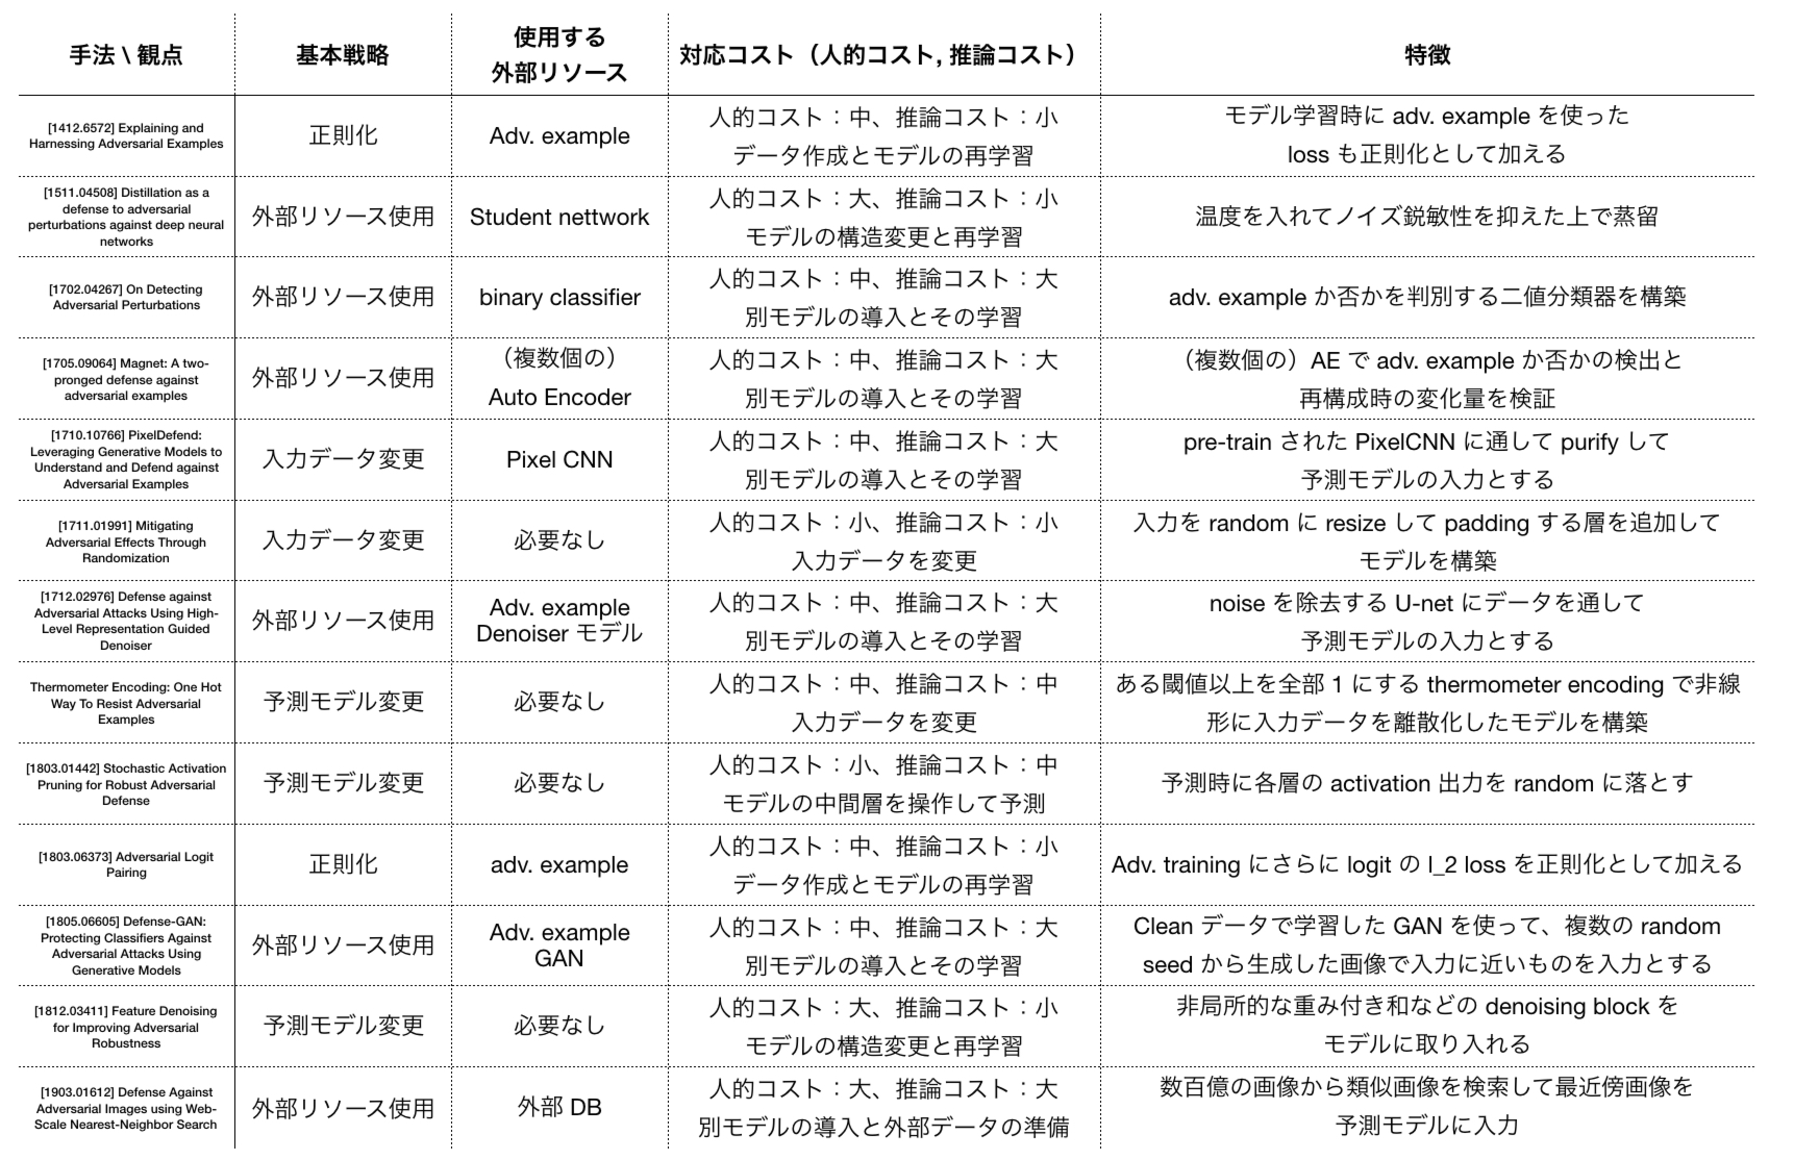
\includegraphics[width=16.0cm]{figures/defense-summary-table.pdf}
\end{center}
\caption{
本書で解説する防御手法の一覧とその特徴をまとめた表.
基本戦略, 使用する外部リソース, 対応コスト, という観点でまとめている.
対応コストは定量的なものではなく, 該当手法の導入に人手の作業がどれくらい発生するかと推論速度への影響がどれくらいかを大まかに評価したものになっていることに注意されたい.
文字が小さいため拡大して見ることを推奨.
}
\label{fig:defense-summary-table}
\end{figure}
%



\subsection{Explaining and Harnessing Adversarial Examples}
\label{subsec:explaining-and}
%
\begin{table}[htbp]
\begin{center}
\begin{tabular}{|c|c|}
\hline
分類の観点 & この手法が該当するもの \\
\hline
基本戦略 & 正則化 \\
使用する外部リソース & adversarial examples \\
対応コスト & 人的コスト:中, 推論コスト:小 \\
\hline
\multicolumn{2}{|c|}{非公式実装: 検証実験のコードに含まれている} \\
\hline
\end{tabular}
\label{tb:explaining-and-summary}
\end{center}
\end{table}
%

FGSM を提案した論文 \cite{goodfellow2014explaining} において、防御方法である adversarial training も同時に提案されている。
アイデアとしては straightforward で, モデルが adversarial examples に対して誤認識をしてしまうならば, その adversarial examples を学習データに含めて学習すればよいという方針である.
これを実現するには何かしらの攻撃手法を導入して adversarial examples を作成する必要があり, その攻撃手法に強く依存した防御手法になっている.

基本戦略は正則化であり, clean なデータを用いた場合の loss に加えて adversarial examples に対する loss も合わせた loss を構成する.
そのため通常の学習で使用するリソース以外にも adversarial examples の分だけ余分にリソースが必要となる.
adversarial examples を作成しそれを含めて学習し直す必要があるので人的コストは中程度掛かるが, 学習後のモデルは adversarial training の有無に依らずに同一なので推論に必要となる余分なコストは発生しない.

定式化は上で述べたことをそのまま実行するだけで, 以下の loss function で学習をすればよい(ここでは単一のデータでの loss function として書いているが, 実際の学習ではミニバッチを使用する).
%
\begin{eqnarray}
\tilde{J} (f, x, y) = \alpha J (f, x, y_{\text{true}}) + (1 - \alpha) J (f, x + \omega, y_{\text{true}}).
\label{eq:explaining-and-loss}
\end{eqnarray}
%
元論文では $\alpha = 0.5$ と $\omega$ を作成する際に FGSM を使用している.
$\omega$ を作成する際には状況に応じて様々な攻撃手法を採用することが可能である

実験は MNIST を用いて実施しており, maxout network \cite{goodfellow2013maxout} に対して $\epsilon = 0.25$ の adversarial examples を作成し, adversarial training なしでは誤認識率が 89.4\% だったが adversarial training ありでは 17.9\% まで減少したと報告されている.

この adversarial training は広く使われている防御手法であるが, \cite{kurakin2016adversarial} で label leaking という問題点が指摘された.
これは少し混乱しやすいので順を追って見ていこう.
まず $f_{\text{label}} (x) \neq y_{\text{true}}$ というデータ $x$ を考える.
この $x$ に対応する $x_{\text{adv}}$ を作成して adversarial training を実施すると, $x$ は当てられなくとも $x_{\text{adv}}$ は当てられるという傾向を持ったモデルが構築され得る.
これはモデルとしては対象物の特徴を捉えるというより摂動のみに注目して予測をするという振る舞いをしてしまうため, テストデータを評価する際に clean なデータは当てられないが adversarial examples は当てやすいという状況を生んでしまう.
そのため, 不当に adversarial examples に対する精度を高めてしまうので正しい評価ができない, という問題である.

この label leaking を防ぐには, 学習の際に $y_{\text{true}}$ を使うのではなく $f_{\text{label}} (x)$ を使えばよい.
これを考慮した loss function は以下のように書ける.
%
\begin{eqnarray}
\tilde{J} (f, x, y) = \alpha J (f, x, y_{\text{true}}) + (1 - \alpha) J (f, x + \omega, f_{\text{label}} (x)).
\label{eq:explaining-and-loss-model-prediction}
\end{eqnarray}
%
これは学習時の話であり, テスト時に adversarial examples を作成するときは $y_{\text{true}}$ を使用すればよい.



\subsection{Distillation as a Defense to Adversarial Perturbations against Deep Neural Networks}
\label{subsec:distillation-as}
%
\begin{table}[htbp]
\begin{center}
\begin{tabular}{|c|c|}
\hline
分類の観点 & この手法が該当するもの \\
\hline
基本戦略 & 外部リソース使用 \\
使用する外部リソース & student network \\
対応コスト & 人的コスト:大, 推論コスト:小 \\
\hline
\multicolumn{2}{|c|}{非公式実装: \href{https://github.com/carlini/nn_robust_attacks}{https://github.com/carlini/nn\_robust\_attacks}} \\
\hline
\end{tabular}
\label{tb:distillation-as-summary}
\end{center}
\end{table}
%

これは \cite{papernot2016distillation} によって提案された手法であり, 蒸留を用いて構築した student network は元のモデルに対する adversarial examples に対して誤認識率が低いということを示した.
蒸留とは図 \ref{fig:distillation-as-summary} のように元のモデル(teacher network と呼ぶ)の出力を用いて蒸留されたモデル(student network と呼ぶ)を学習する手法を指す.
この論文で考えている状況は, 元の学習モデルの情報は攻撃者も知ることができて adversarial examples を作成するが, student network は防御者のみが扱えるもので, この student network は teacher network を基に作成した adversarial examples に対して誤認識しづらいという結果が得られている.
%
\begin{figure}[htbp]
\begin{center}
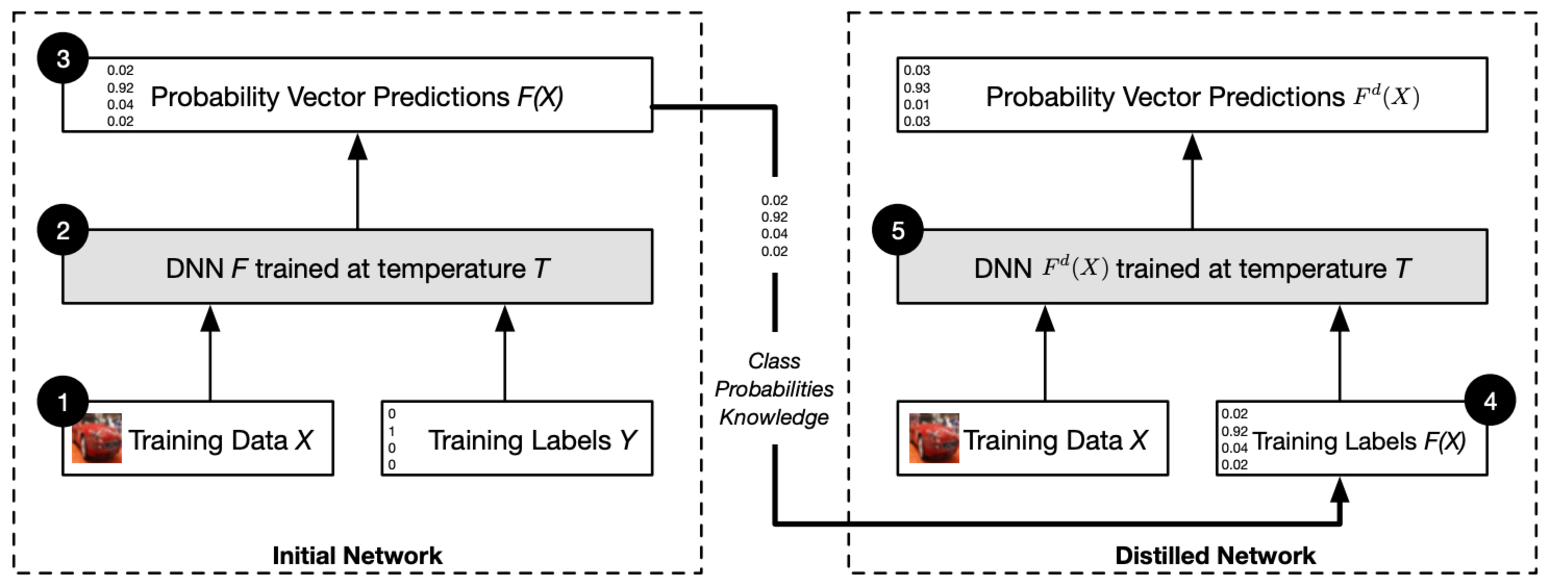
\includegraphics[width=14.0cm]{figures/distillation-as-summary.pdf}
\end{center}
\caption{
蒸留の概念図.
元のモデルの出力を蒸留されたモデルの入力にして学習をする.
この図での $F(X)$ は本書での表記における $f_{\text{prob}}(x)$ に対応している.
図は \cite{papernot2016distillation} より引用.
}
\label{fig:distillation-as-summary}
\end{figure}

基本戦略は外部リソース使用であり, 元のモデルとは独立の student network を準備してそれを学習する必要がある.
student network のアーキテクチャ設計や再学習に係るパラメタ調整など人的コストは大きい.
一方で, 典型的には student network は元のモデルよりも小さく作ることが多いため, 推論のコストは低く, 場合によっては元のモデルよりも速い推論速度を達成し得る.

蒸留自体は adversarial examples とは独立の概念であるため, 詳しくは \cite{hinton2015distilling} などを参照してもらうとして, ここでは蒸留の際に重要となる温度パラメタについて解説をする.
温度パラメタ $T$ とは softmax 値を計算する際に出力確率値がなだらかになるように導入するパラメタである.
%
\begin{eqnarray}
f_{\text{prob}, i} (x) = \frac{e^{f_{\text{logit}, i}(x) / T}}{\sum_{i' = 1}^{C} e^{f_{\text{logit}, i'}(x) / T}}.
\label{eq:distillation-as-temp}
\end{eqnarray}
%
ここでは成分の計算が陽に見えるように $i$ 番目の成分を $f_{\text{prob}, i} (x)$ などと表記している.
この温度パラメタ $T$ が大きいほどクラス毎の確率値の差が小さくなり, より soft な出力になる(T が無限大の極限を取ればどのクラスの出力も $1 / C$ となる).
温度パラメタの導入により, 温度が高い場合に入力の微小な変化の影響を受けづらいという定性的な議論が展開される.
これは $\partial f_{\text{prob}, i} (x) / \partial x_j$ という微分を考えた時に logit が $1/T$ 倍されているので温度パラメタを導入しない場合と比べて変化量が小さくなるためである.
ただし通常は推論時には $T=1$ とするため, ここでの議論は「定性的」であり, 論文でも future work としている.

提案手法は, $T$ を導入して元のモデルを学習した後に $(x, f_{\text{prob}} (x))$ を作成し, それを入力として student network を学習する, というのみである.
student network を $f^d$ と書くことにすると, loss function は以下のようになる.
%
\begin{eqnarray}
J(f, f^d, x) = \sum_{i = 1}^{C} f_{\text{prob}, i} (x) \log f^d_{\text{prob}, i} (x).
\label{eq:distillation-as-loss}
\end{eqnarray}
%

MNIST と CIFAR10 を用いた実験結果に移る.
モデルはそれぞれのデータセットに対して特に工夫を凝らしていない CNN を構築しており, adversarial examples は \cite{papernot2016limitations} で提案された saliency map を使った手法で作成する.
結果は図 \ref{fig:distillation-as-result-table} で, $T$ を高く設定することで誤認識率を減少させることに成功している.
%
\begin{figure}[htbp]
\begin{center}
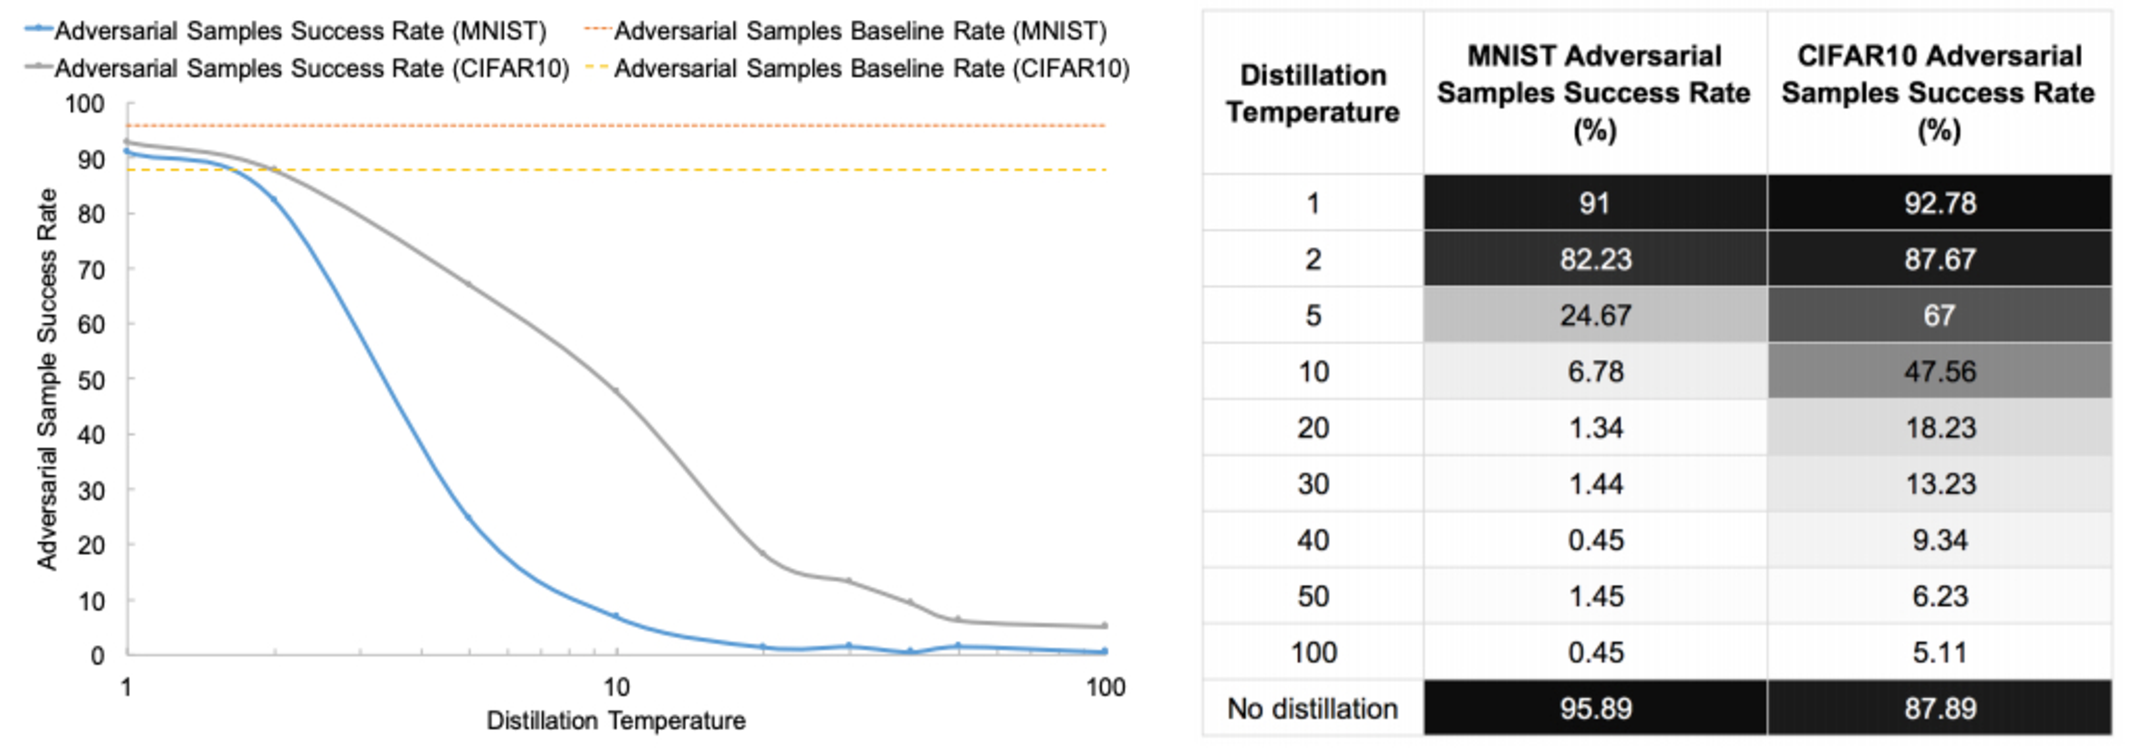
\includegraphics[width=16.0cm]{figures/distillation-as-result-table.pdf}
\end{center}
\caption{
温度パラメタ $T$ と adversarial examples の攻撃成功率の関係性.
$T$ を大きくするほど攻撃成功率が下がり, 防御が成功していることを示している.
図は \cite{papernot2016distillation} より引用.
}
\label{fig:distillation-as-result-table}
\end{figure}
%

また, 図 \ref{fig:distillation-as-diff} にあるように clean データに対する性能の変化も 1.5\% 以内であることも報告している.
MNIST ではどれも精度が下がっているが CIFAR10 では逆に精度が上がる場合もあるため, 蒸留をしたり $T$ を高くすることで必ずしも精度が下がるわけではないことが示されている.
%
\begin{figure}[htbp]
\begin{center}
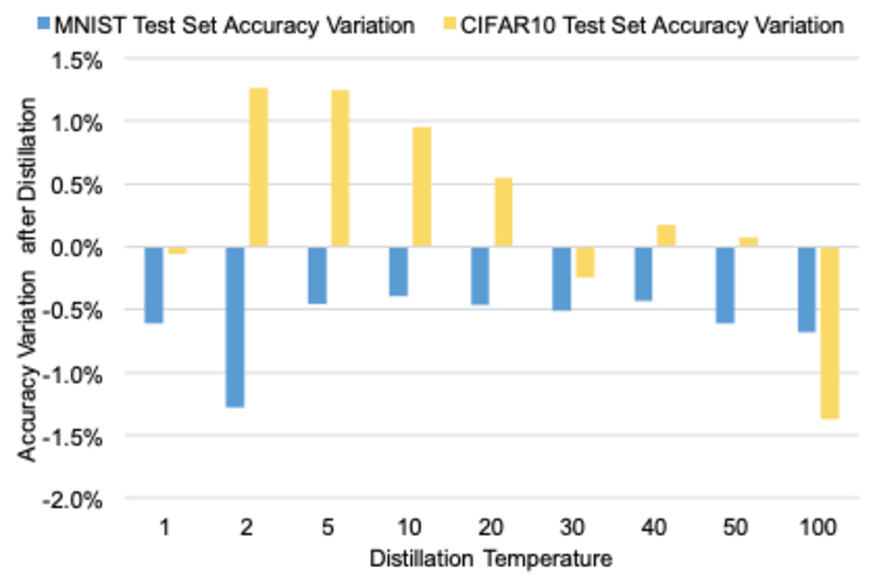
\includegraphics[width=8.0cm]{figures/distillation-as-diff.pdf}
\end{center}
\caption{
蒸留の前後で clean データに対する精度変化を調べた結果.
図は \cite{papernot2016distillation} より引用.
}
\label{fig:distillation-as-diff}
\end{figure}

論文では student network が元のモデルに統計的に近しいことなども議論しているが, 本質的に adversarial examples とは関係がないのでここでは割愛する.

この論文は蒸留を adversarial examples の防御として利用するという点で興味深いが, 状況として攻撃者は元のモデルの情報は取得できるが student network の情報は取得できないという特殊な想定をしている点に注意が必要である.
例えば, inception-v3 \cite{szegedy2016rethinking} のようなよく知られたモデルをそのまま使う場合は攻撃の危険に晒される可能性があり, それを防ぐためにこの手法が利用する, というような使い方が考えられる.



\subsection{On Detecting Adversarial Perturbations}
\label{subsec:on-detecting}
%
\begin{table}[htbp]
\begin{center}
\begin{tabular}{|c|c|}
\hline
分類の観点 & この手法が該当するもの \\
\hline
基本戦略 & 外部リソース使用 \\
使用する外部リソース & binary classifier \\
対応コスト & 人的コスト:中, 推論コスト:大 \\
\hline
\multicolumn{2}{|c|}{非公式実装: \href{https://github.com/carlini/nn_robust_attacks}{https://github.com/carlini/nn\_robust\_attacks}} \\
\hline
\end{tabular}
\label{tb:on-detecting-summary}
\end{center}
\end{table}
%

これは \cite{metzen2017detecting} によって提案された手法であり, 元のモデルとは別の adversarial examples か否かを二値分類する binary classifier を準備するというものである.
図 \ref{fig:on-detecting-model} のように, 元のモデルと同じ入力もしくは元のモデルの中間層出力を binary classifier の入力とする.
FGSM などの基本的な攻撃手法に対して, 元のモデルでは誤認識を引き起こす adversarial examples に対して検出を試み, binary classifier の勾配情報も攻撃者に使われた状況でも探索範囲内の worst case でも 70\% 以上検出できることを示した(二値分類で chance rate が 50\% なので非常に高いというわけではない).
%
\begin{figure}[htbp]
\begin{center}
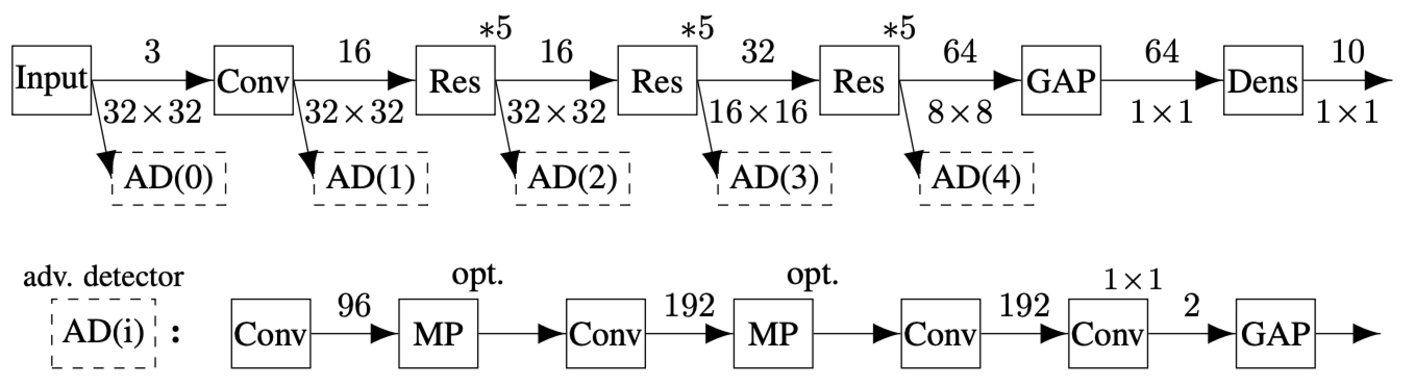
\includegraphics[width=14.0cm]{figures/on-detecting-model.pdf}
\end{center}
\caption{
元のモデルと binary classifier (論文では Adversarial Detector で AD と表記しているが, object detection との混同が生じやすいので本書では binary classifier と表記する) を併用している図.
元のモデルは ResNet を使用しており, Conv は convolution, Res は residual blocks, GAP は global average pooling, Dens は fully connected を意味している.
binary classifier は比較的シンプルなモデルで, 入力として元のモデルと同じ入力や元のモデルの中間層を使う(どれが良いかは実験で決める).
また, MP は max pooling である.
図は \cite{metzen2017detecting} より引用.
}
\label{fig:on-detecting-model}
\end{figure}

基本戦略は外部リソース使用であり, 元のモデルとは独立の binary classifier を準備してそれを学習する必要がある.
binary classifier の設計や学習が必要となるが, モデルはあまり複雑ではないので人的コストは中程度である.
推論時には元のモデルの予測とは別に binary classifier の予測が必要になるため推論コストは大きい(特に元のモデルの中間層出力を使用する場合は中間層出力を得るまでは並列で走らせることもできない).

導入した binary classifier を clean データとその adversarial examples をそれぞれラベル 0, 1 として学習すればよいだけなので, 手法としてはシンプルである.
論文では状況設定として static adversaries と dynamic adversaries を考えており, 前者は攻撃者が元のモデルの情報だけを取得できる場合で後者は binary classifier の情報も取得できる場合としている.
前者は元のモデルの勾配情報を作って adversarial examples を作成すればよいだけで, 後者は binary classifier の勾配情報も用いて adversarial examples を作成する必要がある.
後者に関しては $x_{\text{adv}}$ を adversarial examples ではなく clean データと誤認識させたいので, $x_{\text{adv}}$ ありきでそれをラベル 1 ではないという方向の摂動を作りたいという問題設定になる.
そのため, I+FGSM のように $x_{\text{adv}}$ を逐次的に構成していく方法を念頭に置いており, 以下のように書ける. 
%
\begin{eqnarray}
x_{\text{adv}}^{(t+1)} = \text{clip} ( &&x_{\text{adv}}^{(t)} + \alpha \left[ (1 - \sigma) \cdot \text{sign} \left( \Delta_x J(f, x_{\text{adv}}^{t}, y_{\text{true}}) \right) + \sigma \cdot \text{sign} \left( \Delta_x J(f_{\text{b}}, x_{\text{adv}}^{t}, 1) \right) \right] \nonumber \\
&&, x - \omega, x + \omega ).
\label{eq:on-detecting-adv}
\end{eqnarray}
%
ここで, binary classifier として $f_b$, $\alpha = 0.25$, 元のモデルと binary classifier の寄与を調整するパラメタ $0 \leq \sigma \leq 1$ が導入されている.

実験には CIFAR10 データを用いており, adversarial examples の作成方法として FGSM, I+FGSM, DeepFool を用いている.
まず, static adversaries の結果は図 \ref{fig:on-detecting-static} の通りである.
adversarial examples を使わずに予測させた結果は期待通り 50\% 程度であり, adversarial examples に対しては概ね 80\% 以上の検出率を達成している.
大まかな傾向としては元のモデルを誤認識させやすい adversarial examples ほど binary classifier で検出しやすくなっている.
binary classifier の入力としては元のモデルの入力と出力の中間に位置する中間層出力を使うのが良いという結果が示されている.
これはなかなか解釈が難しいが, モデル依存性が大きいようにも思われる.
%
\begin{figure}[htbp]
\begin{center}
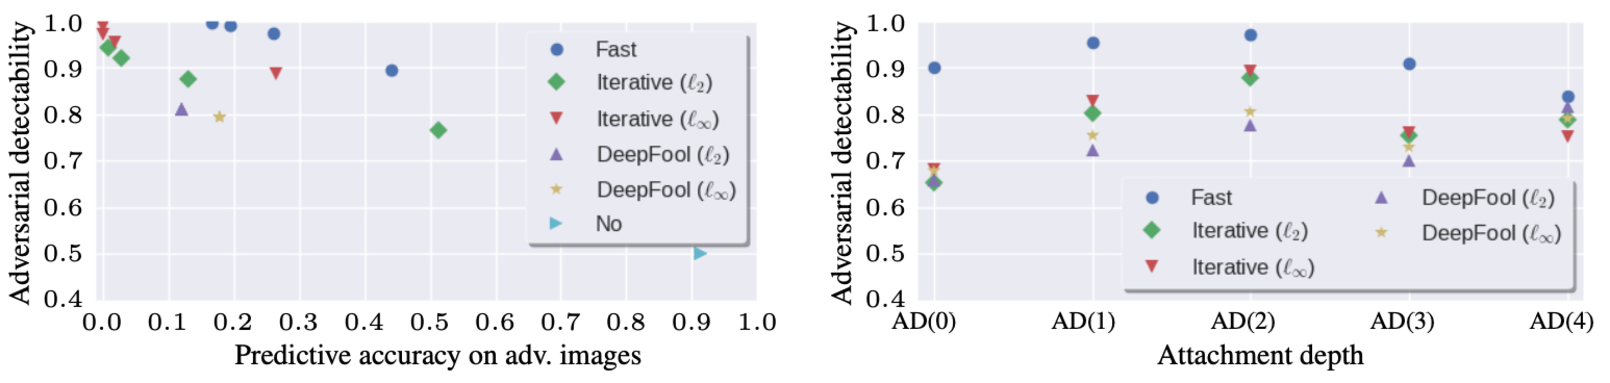
\includegraphics[width=14.0cm]{figures/on-detecting-static.pdf}
\end{center}
\caption{
static adversaries 実験の結果.
左図は縦軸が binary classifier による adversarial examples の検出成功率で, 横軸が元のモデルによる adversarial examples の予測精度である.
$l_{\infty}$ ノルムの上限 $\epsilon$ 様々に変えた結果がプロットされており, 印が左側にいくほど $\epsilon$ が大きい.
右図は縦軸は同じで横軸は binary classifier の入力としてどの情報を使うかである.
図は \cite{metzen2017detecting} より引用.
}
\label{fig:on-detecting-static}
\end{figure}


次に, dynamic adversaries の結果は図 \ref{fig:on-detecting-dynamical-exp} の通りである.
こちらの場合 binary classifier の勾配情報も利用して adversarial examples を作成しているため検出成功率は低下しているが, dynamic では worst case でも 70\% 以上の検出成功率を達成している.
$\sigma$ の値が小さいときは $x_{\text{adv}}$ として元のモデルの勾配情報を重く扱っている場合で, 元のモデルをうまく騙せるものになっているが, その場合 binary classifier で検出しやすくなる.
一方で $\sigma$ の値が大きいときは $x_{\text{adv}}$ として binary classifier の勾配情報を重く扱っている場合で, 元のモデルをうまく騙せなくなっていることに加えて binary classifier での検出成功率も高く保たれているという点は興味深い.
モデルの誤認識率を高めるようにすれば binary classifier で検出しやすくなり, binary classifier を騙そうとし過ぎると元のモデルで誤認識しないばかりか binary classifier を騙すこともできなくなることを示している\footnote{
この部分は自明ではない.
binary classifier に特化するとナイーブには binary classifier を騙しやすい $x_{\text{adv}}$ が作成できるはずだが, 単純な binary classifier では摂動が限定的になってしまって騙しきれないのかもしれないが, 著者はよく知らない.
}.
%
\begin{figure}[htbp]
\begin{center}
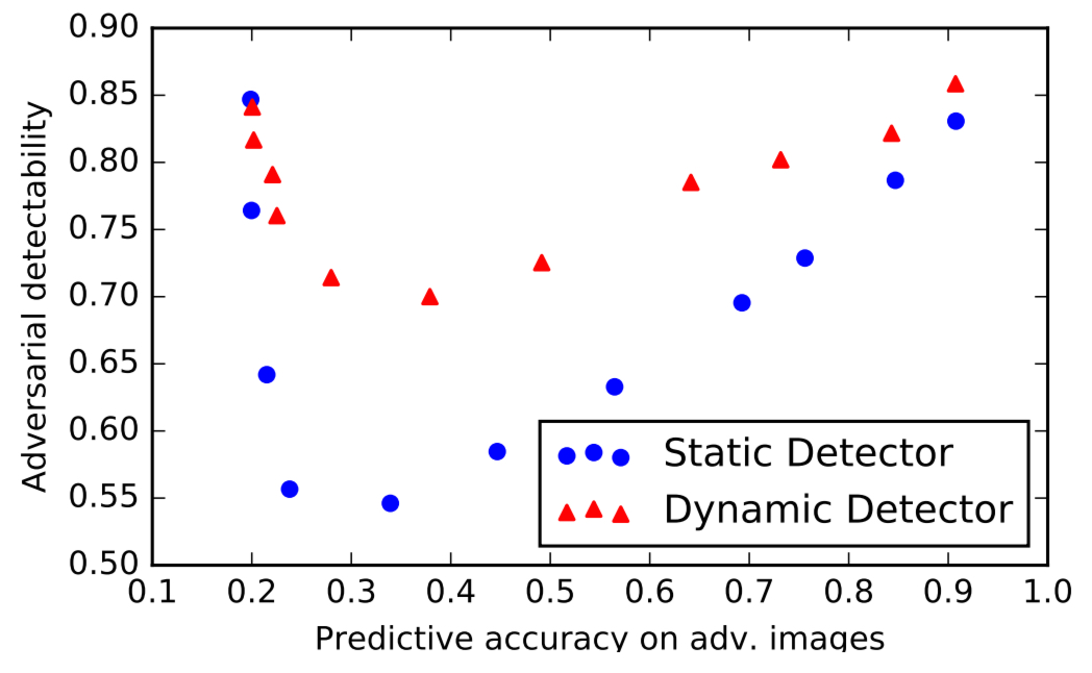
\includegraphics[width=8.0cm]{figures/on-detecting-dynamical-exp.pdf}
\end{center}
\caption{
dynamic adversaries の実験結果.
縦軸は binary classifier による adversarial examples の検出成功率で, 横軸が元のモデルによる adversarial examples の予測精度である.
パラメタ $\sigma$ を $0.1$ 刻みで $[0.0, 1.0]$ の範囲で動かした結果であり, $\sigma$ の値が小さいほど左側の点になる.
青い点は binary classifier の学習に binary classifier の勾配情報を使ってないもので, 赤い点は binary classifier の勾配情報を使ったものである.
$\epsilon = 1 / 255$ で I+FGSM で adversarial examples を作成している.
図は \cite{metzen2017detecting} より引用.
}
\label{fig:on-detecting-dynamical-exp}
\end{figure}

この手法は binary classifier という元のモデルと独立なモデルの導入による防御方法で, adversarial training や元のモデルの中間層の情報を使う場合はそこが密結合となってしまうが, 方向性としては元のモデルとは独立に別のモデルを準備する方向のため導入や削除やアップデートがしやすくなる.
計算資源の面ではコストも低くはないが, 実運用上の方向性しては有望な方向性の一つであろう.



\subsection{MagNet: a Two-Pronged Defense against Adversarial Examples}
\label{subsec:magnet}
%
\begin{table}[htbp]
\begin{center}
\begin{tabular}{|c|c|}
\hline
分類の観点 & この手法が該当するもの \\
\hline
基本戦略 & 外部リソース使用 \\
使用する外部リソース & (複数の) AutoEncoder \\
対応コスト & 人的コスト:中, 推論コスト:大 \\
\hline
\multicolumn{2}{|c|}{公式実装: \href{https://github.com/Trevillie/MagNet}{https://github.com/Trevillie/MagNet}} \\
\hline
\end{tabular}
\label{tb:magnet-summary}
\end{center}
\end{table}
%

これは \cite{meng2017magnet} によって提案された手法であり, 図 \ref{fig:magnet-summary} のようにまずは(一般に複数の)検出器で入力データが adversarial examples か否かを分類し, adversarial examples と分類されなかったものは reformer で正常なデータに近づくように変換して classifier で予測する二段階の仕組みになっている.
検出器の段階では clean なデータから大きく離れる adversarial examples を検出し, それをすり抜けてくる小さな変化量の adversarial examples に対しては clean なデータに戻るように変換をすることで正しい予測をするという戦略となっている.
最も簡単な場合としては, 検出器として AutoEncoder を用いて再構成誤差に閾値を設定して最初の検出を実施し, それをくぐり抜けたデータは同じ AutoEncoder で再構成したデータを入力に予測を実施する.
%
\begin{figure}[htbp]
\begin{center}
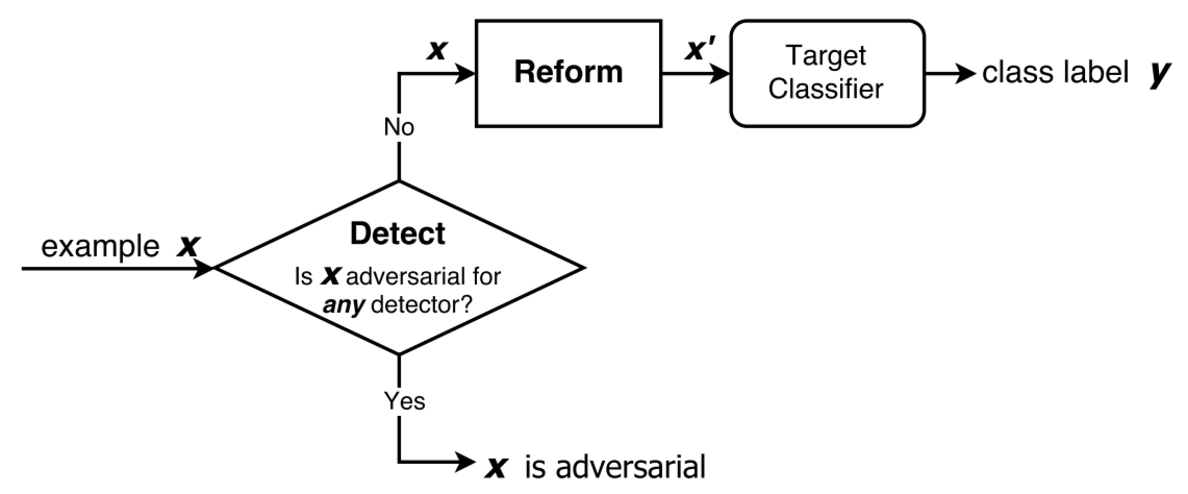
\includegraphics[width=10.0cm]{figures/magnet-summary.pdf}
\end{center}
\caption{
Magnet の概要.
入力データはまず検出器で adversarial examples か否かを分類される.
adversarial examples ではないと分類されたデータは reformer で clean データのサンプルに近づくように変換されるため, 検出器をすり抜けた adversarial examples も正しいラベルと認識されやすくなり, clean データに対しても影響少なく予測できる.
図は \cite{meng2017magnet} より引用.
}
\label{fig:magnet-summary}
\end{figure}


検出器は入力データに対して adversarial examples か否かを分類するものとなり, 一般にはどのようなモデルでもよい.
この論文では後の reformer への使い回しも考慮して, 典型的なものとして AutoEncoder を用いている.
学習は clean データに対する再構成誤差を小さくすることを目的とするため, 以下の loss function を設定する.
%
\begin{eqnarray}
J(AE, x) = \| x - AE(x) \|_2.
\label{eq:magnet-ae-train}
\end{eqnarray}
%
ここで, $AE$ は AutoEncoder であり Encoder のあとに Decoder を適用して $x$ を再構成するものである.
学習した AutoEncoder は推測時には $\|x - AE(x)\|_p$ を計算することで adversarial examples の検出に利用することが可能で, 閾値としては clean データが adversarial examples と分類されてしまう false positive の割合が一定値以下になるように設定する(学習や閾値設定には adversarial examples を用いない).

検出器をもう少し発展させて予測モデルの logit 出力に対する $x$ と $AE(x)$ の divergence を用いるということもできる.
adversarial examples は $x$ の空間では近くても $f_{\text{logit}} (x)$ の空間では遠いものなので, それを利用するアプローチである.
logit から softmax 値を計算して確率値として, 以下のように Jensen-Shannon divergence を計算する.
%
\begin{eqnarray}
JSD(f_{\text{prob}} (x)\|f_{\text{prob}} (AE(x))) &=& \frac{1}{2} D_{KL} \left(f_{\text{prob}} (x) \| \frac{f_{\text{prob}} (x) + f_{\text{prob}} (AE(x)) }{2} \right) \nonumber \\
&+& \frac{1}{2} D_{KL} \left(f_{\text{prob}} (AE(x)) \| \frac{f_{\text{prob}} (x) + f_{\text{prob}} (AE(x)) }{2} \right).
\label{eq:magnet-jsd-ae}
\end{eqnarray}
%
ここで $D_{KL}$ は Kullback-Leibler divergence である.
これも分類時には閾値が必要となるが, 先ほどと同じように clean データのみを用いて false positive が一定値以下になるように定める.
$x$ と $AE(x)$ それぞれの softmax 値が同じ最大要素のみでほぼ 1 になると $JSD$ の値は 0 に近づき違いが見えづらくなるため, 数値的なテクニックとして式 \ref{eq:distillation-as-temp} と同様に温度パラメタを導入する.

一方で reformer としても AutoEncoder を使用する.
これも clean データの再構成誤差で学習し, 一段目の検出器をすり抜けてきた adversarial examples を clean なデータ分布のサンプルとして再構成する方向に働くため, それを classifier の入力とすることで正しい予測が得られると期待される.

実験は MNIST と CIFAR10 で実施している.
予測モデルは特に変わったところのない convolution と ReLU と max pooling や gloval average pooling のモデルのためここでは説明は割愛する.
検出器や reformer は MNIST に関しては図 \ref{fig:magnet-mnist} のように構成していて検出器を 2 つ準備しており\footnote{
MNIST は簡単なデータセットであるため CIFAR10 のように 1 つの検出器と reformer でよい気がするが, なぜ検出器を 2 つ準備しているのかは著者は知らない.
}, CIFAR10 に関しては図 \ref{fig:magnet-cifar10} のように構成している\footnote{
CIFAR10 は decoder の最後の convolution のチャンネル数が 1 になっているが, これは論文の誤植で 3 だと思われる.
}.
検証のための adversarial examples の作成手法としては, FGSM, I+FGSM, Deepfool, Carlini の方法\footnote{
これは loss function を設定してそれに基づいて摂動を求める手法で, 以下の loss function を用いる.
%
\begin{eqnarray}
\min_{\omega} \left[ \|\omega\|_p + c \cdot \max (f_{\text{logit}, y_{\text{true}}} (x_{\text{adv}}) - \max (\{ f_{\text{logit} (x_{\text{adv}}), i} : i \neq y_{\text{true}} \}), - \kappa) \right].
\label{eq:magnet-adv-cw}
\end{eqnarray}
%
さらに $x + \omega \in [0, 1]^m$ となるよう制限する.
これは正しいラベルの logit の値がそれ以外の logit で最大値のものと比べて十分小さくなるように摂動を作成するもので, それだけを目的にするとモデルに特化しすぎて transferability が低くなるため $- \kappa$ で制限している.
FGSM とは異なりこの loss を用いて optimizer を用いて最適化することで所望の摂動を得る.
}, \cite{carlini2017towards} を用いている.
%
\begin{figure}[htbp]
\begin{center}
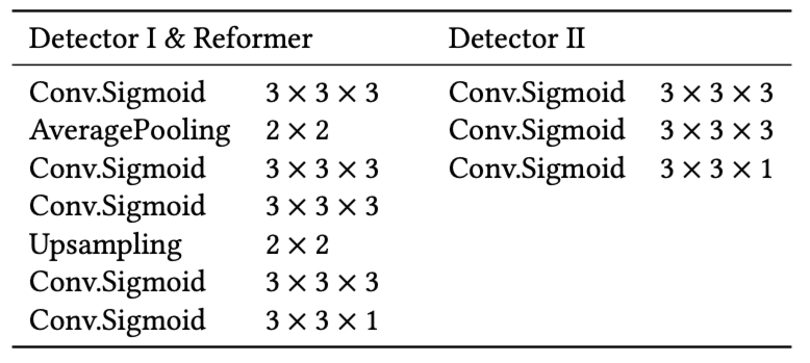
\includegraphics[width=10.0cm]{figures/magnet-model-mnist.pdf}
\end{center}
\caption{
MNIST に対する検出器と reformer の構成.
検出器は 2 つ準備している.
convolution は出力後に入力サイズと同じになるように padding する.
図は \cite{meng2017magnet} より引用.
}
\label{fig:magnet-mnist}
\end{figure}
%
\begin{figure}[htbp]
\begin{center}
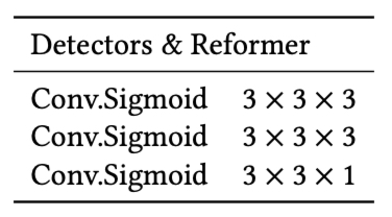
\includegraphics[width=6.0cm]{figures/magnet-model-cifar10.pdf}
\end{center}
\caption{
CIFAR10 に対する検出器と reformer の構成.
同一の AutoEncoder を用いている.
convolution は出力後に入力サイズと同じになるように padding する.
図は \cite{meng2017magnet} より引用.
}
\label{fig:magnet-cifar10}
\end{figure}


MNIST の結果は図 \ref{fig:magnet-result-mnist} の通りである.
検出器は Jansen-Shannon divergence は用いずに再構成誤差のみを用いており, 閾値としては validation セットに対する false positive が 0.1\% になるように定めている.
CW の方法では元のモデルでは全く正答することができていないが, MagNet によって 90\% を超える精度を達成している.
また, clean テストデータに対しては MagNet なしでは 99.4\% であり MagNet ありでは 99.1\% であり影響が少ないことが示されている.
%
\begin{figure}[htbp]
\begin{center}
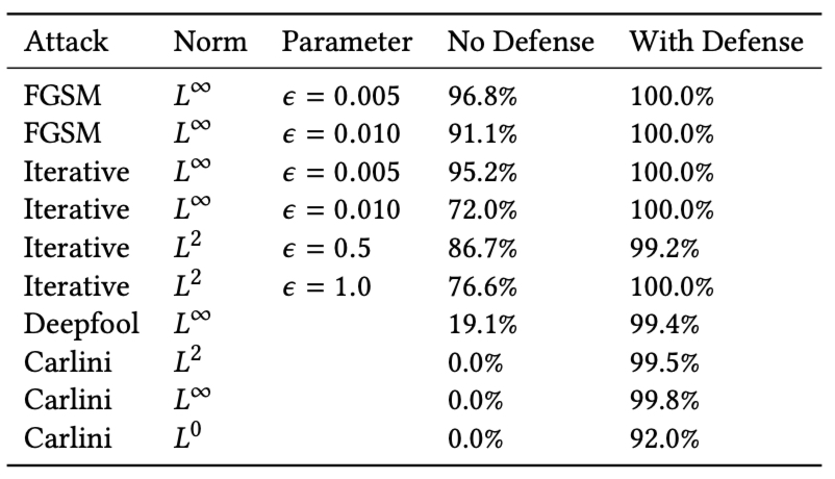
\includegraphics[width=10.0cm]{figures/magnet-result-mnist.pdf}
\end{center}
\caption{
防御手法の有無による MNIST のテストデータに対する精度の違い.
精度は clean データに対して正答することができるものがを adversarial examples に差し替えた場合の精度を示している.
防御手法のうち検出器は Jansen-Shannon divergence は用いずに再構成誤差のみを用いている.
攻撃は予測モデルの情報だけを使える状況設定で MagNet に対する情報は用いていない.
図は \cite{meng2017magnet} より引用.
}
\label{fig:magnet-result-mnist}
\end{figure}
%

CIFAR10 の結果は図 \ref{fig:magnet-result-cifar10} の通りである.
検出器は再構成誤差だけではなく Jansen-Shannon divergence も用いており, 温度パラメタは $T=10, 40$ の 2 つの場合を併用している.
MNIST と比べるとうまく防御できない場合が増えているが, それでもMagNet によって 75\% を超える精度を達成している.
ただし, clean テストデータに対しては MagNet なしでは 90.6\% であり MagNet ありでは 86.8\% であり若干の影響が出ている.
%
\begin{figure}[htbp]
\begin{center}
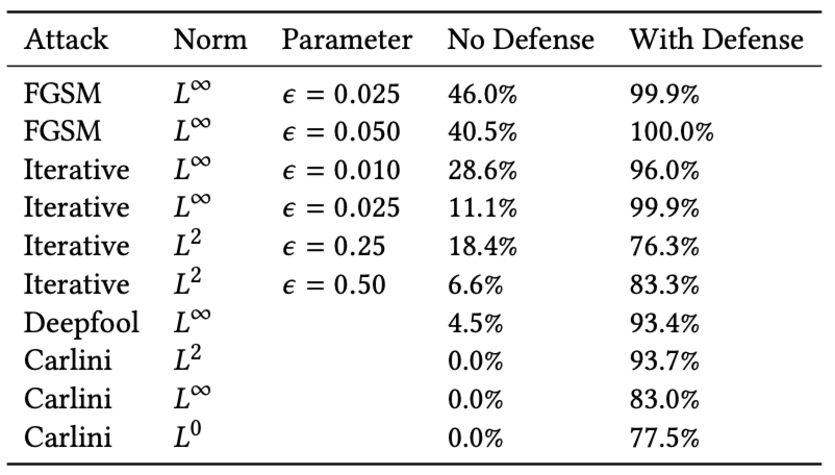
\includegraphics[width=10.0cm]{figures/magnet-result-cifar10.pdf}
\end{center}
\caption{
防御手法の有無による CIFAR10 のテストデータに対する精度の違い.
精度は clean データに対して正答することができるものがを adversarial examples に差し替えた場合の精度を示している.
防御手法のうち検出器は再構成誤差と $T=10, 40$ の場合の Jansen-Shannon divergence を併用している.
攻撃は予測モデルの情報だけを使える状況設定で MagNet に対する情報は用いていない.
図は \cite{meng2017magnet} より引用.
}
\label{fig:magnet-result-cifar10}
\end{figure}
%

この手法は検出器と reformer という 2 つの組み合わせで防御性能を高めたものであるが, 特に reformer で入力画像を clean データ分布に近いものに変換するという考えが興味深いものであった.
この手法以降, 様々な方法で adversarial examples の摂動の効果を除去して正しく予測できるようにする研究が発展した.
ただし, 入力画像の変更は clean データの場合にモデルの degradation を引き起こす恐れもあるので注意が必要である.



\subsection{PixelDefend: Leveraging Generative Models to Understand and Defend against Adversarial Examples}
\label{subsec:pixeldefend}
%
\begin{table}[htbp]
\begin{center}
\begin{tabular}{|c|c|}
\hline
分類の観点 & この手法が該当するもの \\
\hline
基本戦略 & 外部リソース使用 \\
使用する外部リソース & PixelCNN \\
対応コスト & 人的コスト:中, 推論コスト:大 \\
\hline
\multicolumn{2}{|c|}{公式実装: \href{https://github.com/microsoft/PixelDefend}{https://github.com/microsoft/PixelDefend}} \\
\hline
\end{tabular}
\label{tb:pixeldefend-summary}
\end{center}
\end{table}
%

これは \cite{song2017pixeldefend} によって提案された手法であり, 元のモデルとは別の clean データで pre-train された pixelCNN を導入し, 入力データを purify することで摂動の効果を弱めて誤認識を防ぐ.

基本戦略は外部リソースの使用で, pixelCNN を用いる.
別のモデルを準備しなければならないので人的コストは中程度で, 推論は先に pixelCNN を通してから元の予測モデルを適用するのでコストは大きい.

pixelCNN \cite{oord2016pixel, salimans2017pixelcnn++} は画像用に考案された tractable な尤度を基にした生成モデルである.
同時確率分布は以下のように定義される.
%
\begin{eqnarray}
p_{\text{CNN}} (x) = \prod_{i} p_{\text{CNN}} (x_i | x_{1:i-1}).
\label{eq:pixeldefend-pixelcnn-joint-distrib}
\end{eqnarray}
%
これを $- \log \left( p_{\text{CNN}} (x) \right) / (m \times \log 2)$ としたものを bits per dimension と呼び, モデルの評価によく用いられる.
ここではかなり簡略化して書いてあるが, 実際には未来方向の情報を mask した convolution を使ってコンテキストを取得して未来方向のピクセルを予測していく.
pixelCNN は予測するピクセルを softmax 値を用いて選択するモデルになっているため, どのピクセル値がどれくらいの確率であるかが tractable になっているため, 入力データを実現する同時確率が計算可能である.

すなわち clean データで学習した pixelCNN があれば, 入力データの同時確率を計算することでその確率が高ければ clean データで低ければ adversarial examples であると分類できる.
これは統計的な枠組みで議論できる.
clean データ $x^{(1)}, x^{(2)}, \dots x^{(N)}$ を iid で確率分布 $p (\mathcal{X})$ からサンプルされたものだとする.
対象となるデータ $x_{\text{adv}}$ が iid で確率分布 $p (\mathcal{X_{\text{adv}}})$ からサンプルされたものだとして, 帰無仮説として $p (\mathcal{X}) = p (\mathcal{X_{\text{adv}}})$ を採用して対立仮説として $p (\mathcal{X}) \neq p (\mathcal{X_{\text{adv}}})$ を採用する.
統計量 $T$ を以下のように定義する.
%
\begin{eqnarray}
T = T(x_{\text{adv}}; x^{(1)}, x^{(2)}, \dots x^{(N)}) = \sum_{i=1}^{N} \mathbb{I} \left[ p_{\text{CNN}} (x^{(i)}) \leq p_{\text{CNN}} (x_{\text{adv}}) \right].
\label{eq:pixel-defend-pixelcnn-test-stat}
\end{eqnarray}
%
ここで $\mathbb{I} [\cdot]$ は indicator function で括弧内の条件が true なら 1 でそうでなければ 0 を返す.
あとは $T^{(i)} = T(x^{(i)}; x^{(1)}, \dots, x^{(i-1)}, x_{\text{adv}}, x^{(i+1)}, \dots, x^{(N)})$ として permutation test を実施すればよい.
具体的には p 値が以下で計算される.
%
\begin{eqnarray}
p = \frac{1}{N + 1} \left( \sum_{i=1}^{N} \mathbb{I} [T_i \leq T] + 1 \right) = \frac{T + 1}{N + 1}.
\label{eq:pixel-defend-pixelcnn-test-pvalue}
\end{eqnarray}
%

以上が adversarial examples を検出する仕組みであったが, もう一歩進めて pixelCNN を入力データを purify するために用いて正しい予測を実施するという手法も提案されている.
これは clean データで学習した pixelCNN が出力として clean データの分布に従うピクセル値を出力しやすいという性質を利用したもので, アルゴリズム \ref{alg:pixeldefend-alg} にその手順を示す.
%
\begin{algorithm}
\caption{pixelCNN によるデータ purification のアルゴリズム}
\label{alg:pixeldefend-alg}
\begin{algorithmic}[1]
    \State Input: 入力データ $x$, パラメタ $\epsilon_{\text{defend}}$, 学習済みの pixelCNN $p_{\text{CNN}}$.
    \State Output: purify されたデータ $x_{\text{purified}}$.
	\State 出力を初期化: $x_{\text{purified}} \leftarrow x$
	\For {各ピクセル $x_i \in \mathcal{X}$}
	\State 出力範囲を設定: $R \leftarrow \left[ \max (x_i - \epsilon_{\text{defend}}, 0), \min (x_i + \epsilon_{\text{defend}}, 255) \right]$.
	\State $x_{\text{purified}, i}$ に対応する pixelCNN の出力を計算: $o = \prod_{i'}^i p_{\text{CNN}} (x_{\text{purified}, i'} | x_{\text{purified}, 1:i' - 1})$.
	\State $x_{\text{purified}}$ の要素を更新: $x_{\text{purified}, i} \leftarrow \argmax_{z \in R} \left[ o[z] \right]$.
    \EndFor
\end{algorithmic} 
\end{algorithm}
%

実験は CIFAR10 で実施しており, 攻撃方法は RAND, FGSM, I+FGSM, DeepFool, CW の方法, を用いている.
p 値の分布は図 \ref{fig:pixeldefend-pvalue} で, 画像を purify した例は図 \ref{fig:pixeldefend-purification} である.
どちらも期待通りの挙動を示している.
%
\begin{figure}[htbp]
\begin{center}
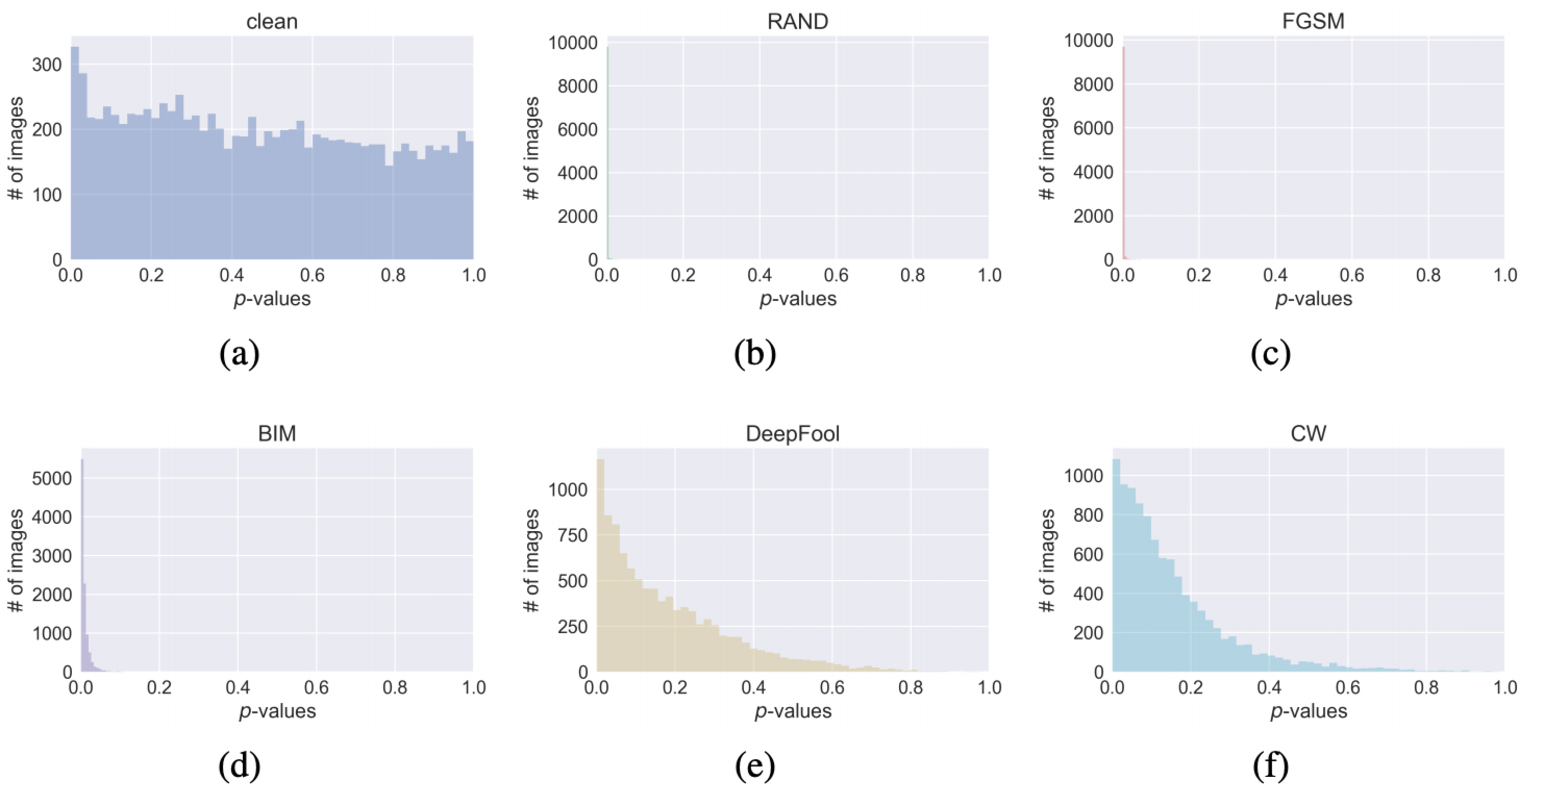
\includegraphics[width=14.0cm]{figures/pixeldefend-pvalue.pdf}
\end{center}
\caption{
pixelCNN で CIFAR10 に対して算出した p 値.
BIM は I+FGSM と同一である.
縦軸のスケールは攻撃手法毎に異なる.
図は \cite{song2017pixeldefend} より引用.
}
\label{fig:pixeldefend-pvalue}
\end{figure}
%
\begin{figure}[htbp]
\begin{center}
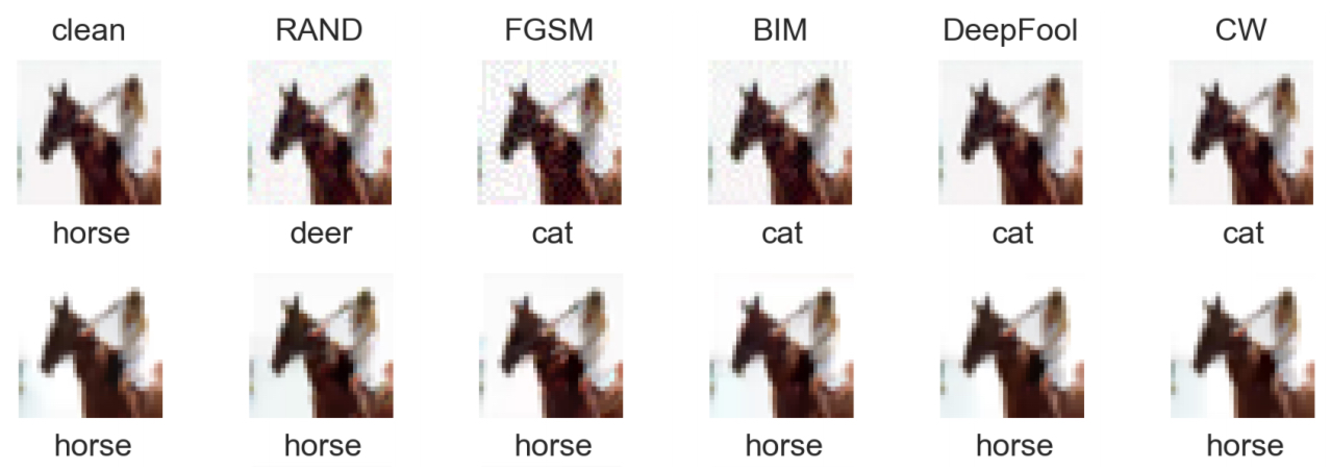
\includegraphics[width=14.0cm]{figures/pixeldefend-purification.pdf}
\end{center}
\caption{
pixelCNN で CIFAR10 のデータに対して purifaction を実施した例
BIM は I+FGSM と同一である.
画像の下のラベルは clean データで学習した ResNet での予測結果で, purify したデータでは全て正しく予測できている.
図は \cite{song2017pixeldefend} より引用.
}
\label{fig:pixeldefend-purification}
\end{figure}

提案手法の性能を定量的に実験した結果が図 \ref{fig:pixeldefend-cifar10} である.
提案手法は結果が安定していることが読み取れる.
単体では従来手法を上回るほどではないが, 従来手法と組み合わせることで特に性能が高い攻撃手法に対しては adversarial training と比べて良い結果を示している.
また, 組み合わせることで clean data に対する degradation も軽減している.
%
\begin{figure}[htbp]
\begin{center}
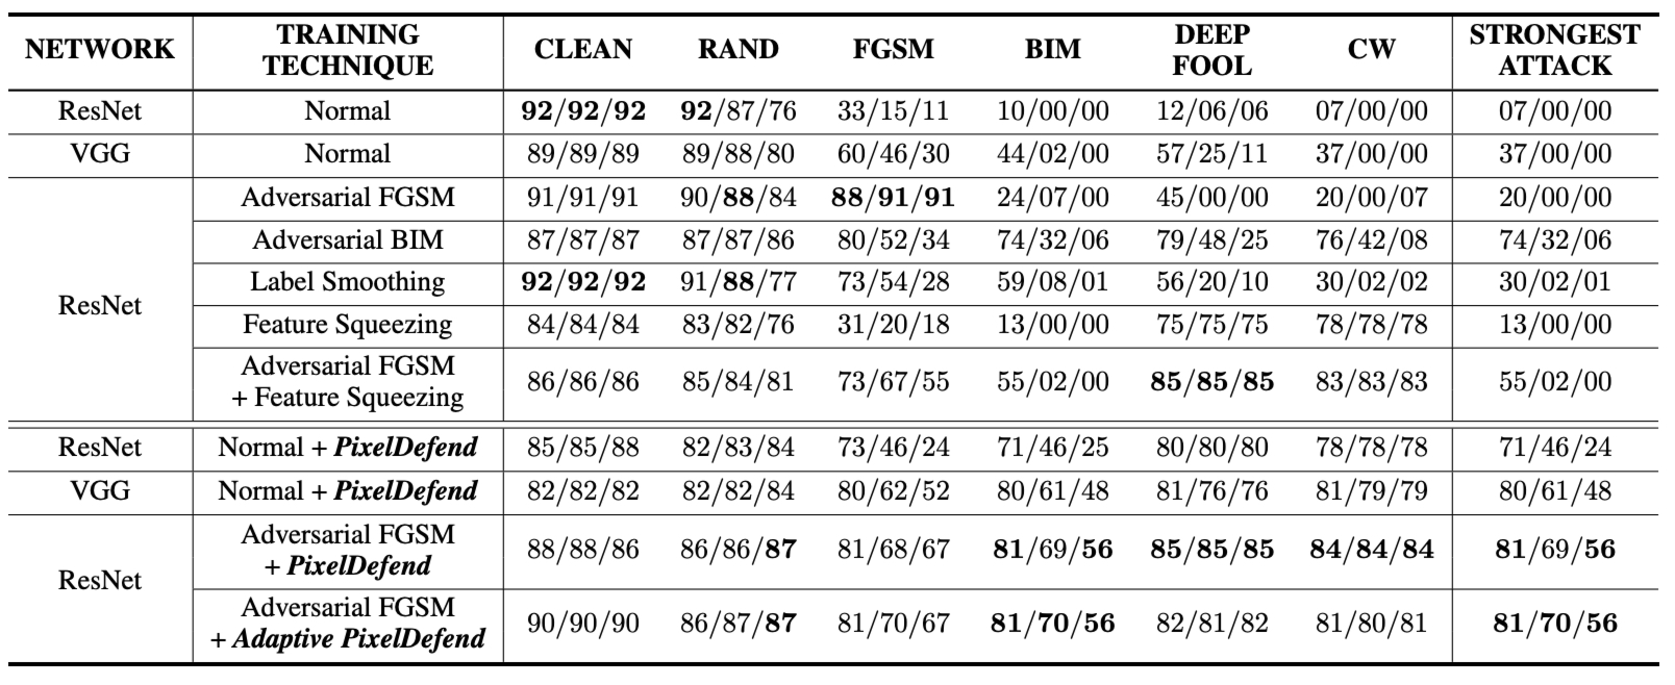
\includegraphics[width=14.0cm]{figures/pixeldefend-cifar10.pdf}
\end{center}
\caption{
CIFAR10 のテストデータに対する実験結果.
3 つ数字があるのは adversarial examples として $\epsilon = 2/255, 8/255, 16/255$ それぞれの結果である.
$\epsilon_{\text{defend}} = 16/255$ を用いている.
STRONGEST ATTACK は最も精度が低い攻撃手法の結果である.
Adaptive PixelDefend は $\epsilon_{\text{defend}}$ を攻撃方法に合わせて適した値を手で設定しているものである.
図は \cite{song2017pixeldefend} より引用.
}
\label{fig:pixeldefend-cifar10}
\end{figure}

この手法は pixelCNN を画像の purification に用いたという点が新しいものであった.
MagNet と同様に clean データで学習したモデルを用いて入力データを変換すると adversarial examples が clean データに近づくという性質を利用しており, 他手法と比べることで degradation も抑えられている.
同様のアイデアの手法としては \cite{mustafa2019image} などもある.



\subsection{Mitigating Adversarial Effects Through Randomization}
\label{subsec:mitigating-adversarial}
%
\begin{table}[htbp]
\begin{center}
\begin{tabular}{|c|c|}
\hline
分類の観点 & この手法が該当するもの \\
\hline
基本戦略 & 入力データ変更 \\
使用する外部リソース & なし \\
対応コスト & 人的コスト:小, 推論コスト:中 \\
\hline
\multicolumn{2}{|c|}{公式実装: \href{https://github.com/cihangxie/NIPS2017_adv_challenge_defense}{https://github.com/cihangxie/NIPS2017\_adv\_challenge\_defense}} \\
\hline
\end{tabular}
\label{tb:mitigating-adversarial-summary}
\end{center}
\end{table}
%

これは \cite{xie2017mitigating} によって提案された手法であり, 図 \ref{fig:mitigating-adversarial-summary} のように入力データを小さくリサイズしてから元の画像サイズと同じサイズになるように padding したものを改めて入力データとすることで誤認識を防ぐものである.
%
\begin{figure}[htbp]
\begin{center}
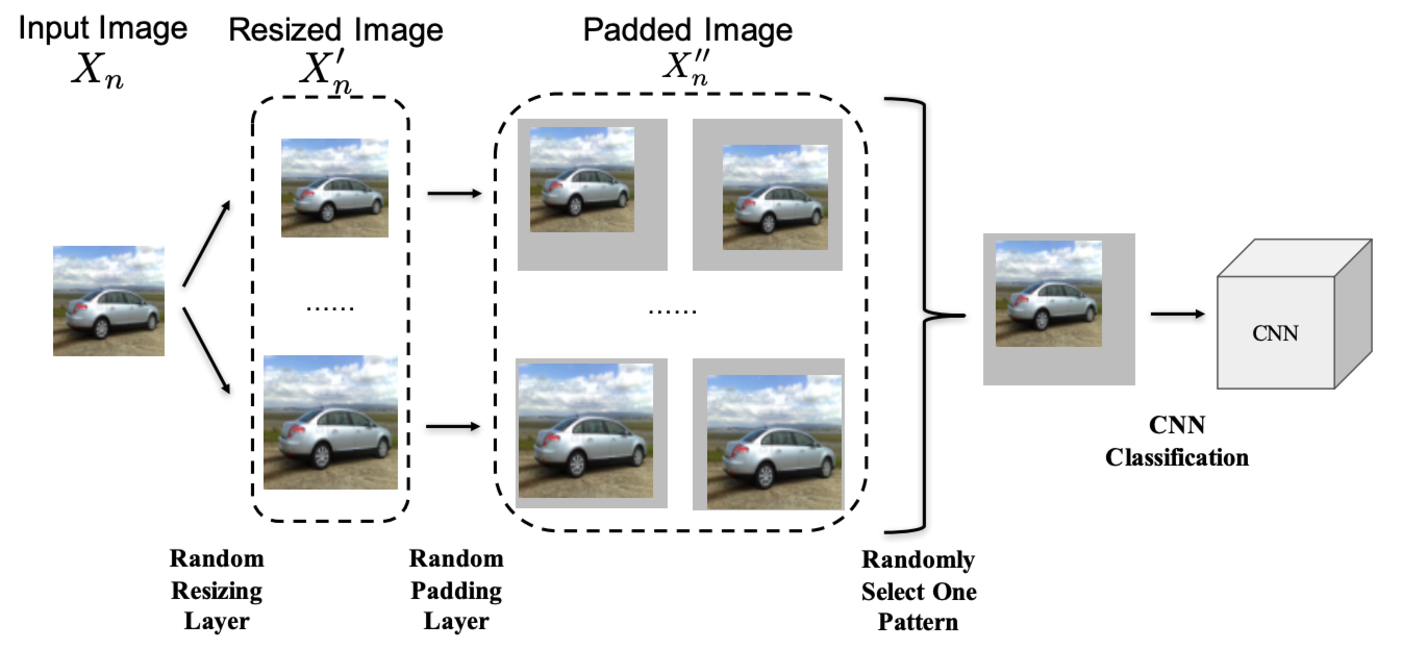
\includegraphics[width=14.0cm]{figures/mitigating-adversarial-summary.pdf}
\end{center}
\caption{
提案手法の概要.
入力データをランダムにリサイズした後, それを一定のサイズになるように 0 padding したものをモデル予測の入力とする.
図は \cite{xie2017mitigating} より引用.
}
\label{fig:mitigating-adversarial-summary}
\end{figure}

基本戦略は入力データ変更で, 摂動の効果が弱まるようにリサイズや 0-padding を用いる.
外部リソースが必要なく, コストが低いのが特徴である.

手法としてはシンプルである.
入力データサイズを [299, 299, 3] の場合を想定しており, まず resize として $rnd \in$ [299, 331) を用いて [$rnd$, $rnd$, 3] とする.
そして 0 埋めした [331, 331, 3] に収まるように resize した画像を配置するというものになっている.
adversarial examples が入力となった場合には, リサイズと 0 padding によって摂動の効果が増幅して誤認識につながることを防ぐというメカニズムである.

実験は, データは ILSVRC2012 の validation セットからランダムにサンプルした 5,000 枚を用いて, adversarial examples の生成は FGSM, DeepFool, CW を用いている.
攻撃対象のモデルは inception-v3, ResNet-v2-101, Inception-ResNet-v2, ens-adv-Inception-ResNet-v2 (ensemble adversarial training と提案手法を併用したもの) としている.
提案手法を導入することによって clean データに対する degradation の可能性が生じるが, 精度劣化は上で紹介したモデルの順に絶対値で 2.7\%, 1.7\%, 0.7\%, 0.8\% でありかなり抑えられている.

まず, 攻撃者が予測モデルの情報だけにアクセスできる場合を考える.
攻撃者はリサイズは 0 padding の存在を知らないため, [299, 299, 3] の入力データを予測モデルの勾配情報を用いて adversarial examples を作成する.
防御側はその adversarial examples をリサイズして 0 padding したものに差し替えて予測する.
その結果が図 \ref{fig:mitigating-adversarial-vanilla} であり, どの攻撃手法に対しても精度が上がっていることが確認できる.
特に DeepFool や CW のように元のモデルに対する攻撃性能が高い手法に対して高い防御性能を発揮している.
これは, FGSM は勾配情報を一度使うだけで「粗い」摂動だが, 高い攻撃性能を誇る攻撃手法はモデルの勾配情報を繰り返し使って摂動の効果が増幅されるように摂動を細かくチューニングするようなもので, チューニングしている分リサイズや 0 padding で位置がずれるとモデルの演算による増幅が生じなくなるためだと考えられる.
%
\begin{figure}[htbp]
\begin{center}
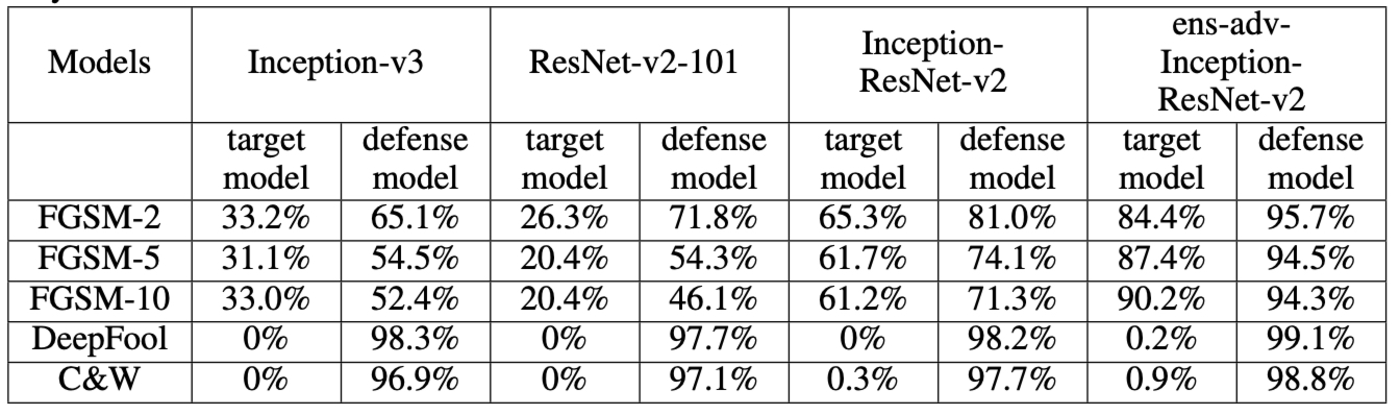
\includegraphics[width=14.0cm]{figures/mitigating-adversarial-vanilla.pdf}
\end{center}
\caption{
攻撃者がリサイズや 0 padding の存在を知らずに入力データと予測モデルの勾配情報のみで adversarial examples を作成した場合.
target model の列はリサイズと 0 padding を使わずに予測モデルに直接 adversarial examples を入力した場合の精度を表す.
defense model の列はリサイズと 0 padding を使った場合の精度を表す.
図は \cite{xie2017mitigating} より引用.
}
\label{fig:mitigating-adversarial-vanilla}
\end{figure}
%

次に, 攻撃者がリサイズや 0 padding の存在を知っていてその情報も用いて攻撃する場合を考える.
しかしながら, 防御手法にはランダム性が含まれているため, 攻撃者にできることは同じ機構で画像を複数生成してそれらを使って adversarial examples を作成するのみである.
リサイズと 0 padding のランダム性を考慮すると可能なパターンは以下の通り 12,528 パターンである.
%
\begin{eqnarray}
\sum_{rnd = 299}^{330} (331 - rnd + 1)^2 = 12528.
\label{eq:mitigating-adversarial-all-patterns}
\end{eqnarray}
%
これを全て生成して adversarial examples を作成するのは大変なので, 合計 21 パターンの画像を生成して精度を調べた結果が図である.
リサイズと 0 padding の情報を使った攻撃に対してはやはり精度は下がるものの, 防御手法としては機能しており特に DeepFool や CW に対しては高い防御性能を保っている.
一方で, FGSM 系に対しては精度はかなり落ちており, これは「粗い」摂動の ensemble 効果によるものだと考えられる.
%
\begin{figure}[htbp]
\begin{center}
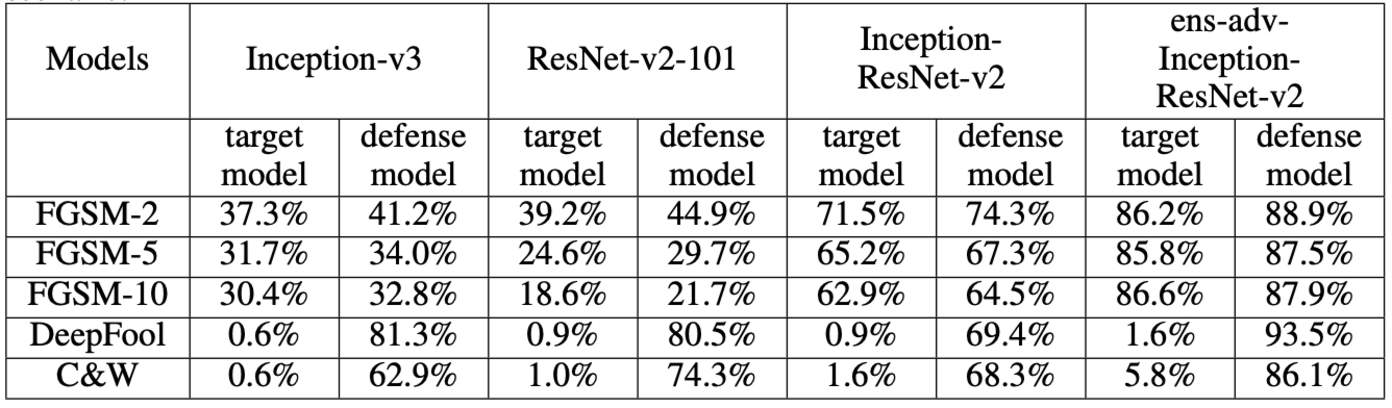
\includegraphics[width=14.0cm]{figures/mitigating-adversarial-ensemble.pdf}
\end{center}
\caption{
攻撃者がリサイズと 0 padding の情報も用いて adversarial examples を作成した場合.
リサイズとして \{299, 307, 315, 323, 331\} の 5 パターン, それを \{中央, 左上, 右上, 左下, 右下\} にセットして 0 padding する合計 $5*4 + 1 = 21$ パターンの画像から adversarial examples を作成(331 の場合は中央にのみセット可能).
target model の列はリサイズと 0 padding を使わずに予測モデルに直接 adversarial examples を入力した場合の精度を表す.
defense model の列はリサイズと 0 padding を使った場合の精度を表す.
図は \cite{xie2017mitigating} より引用.}
\label{fig:mitigating-adversarial-ensemble}
\end{figure}

この手法は入力画像を変更するのみで, 学習済みのモデルへの影響が少なく外部リソースも必要としない低コストな手法であることが
利点である.
ランダム性を取り入れることは adversarial examples に対する有力な防御手段であることが示された.
他の防御手法と組み合わせやすいというのも実用上は重要な点である.



\subsection{Defense against Adversarial Attacks Using High-Level Representation Guided Denoiser}
\label{subsec:defense-against}
%
\begin{table}[htbp]
\begin{center}
\begin{tabular}{|c|c|}
\hline
分類の観点 & この手法が該当するもの \\
\hline
基本戦略 & 外部リソース利用 \\
使用する外部リソース & U-net \\
対応コスト & 人的コスト:中, 推論コスト:大 \\
\hline
\multicolumn{2}{|c|}{公式実装: \href{https://github.com/lfz/Guided-Denoise}{https://github.com/lfz/Guided-Denoise}} \\
\hline
\end{tabular}
\label{tb:defense-against-summary}
\end{center}
\end{table}
%

これは \cite{liao2018defense} によって提案された手法であり, 図 \ref{fig:defense-against-summary} のように摂動を denoise する($x_{\text{adv}} + (- \omega) = x$ を実現する) U-net \cite{ronneberger2015u} を導入して防御する.
DAE のように clean なデータを再現しようとするとするのではなく, 摂動部分のみに注目することでより摂動を認識して対処しようという狙いである.
この手法は NIPS2017 の adversarial examples の competition において防御手法で一位を獲得した手法である.
%
\begin{figure}[htbp]
\begin{center}
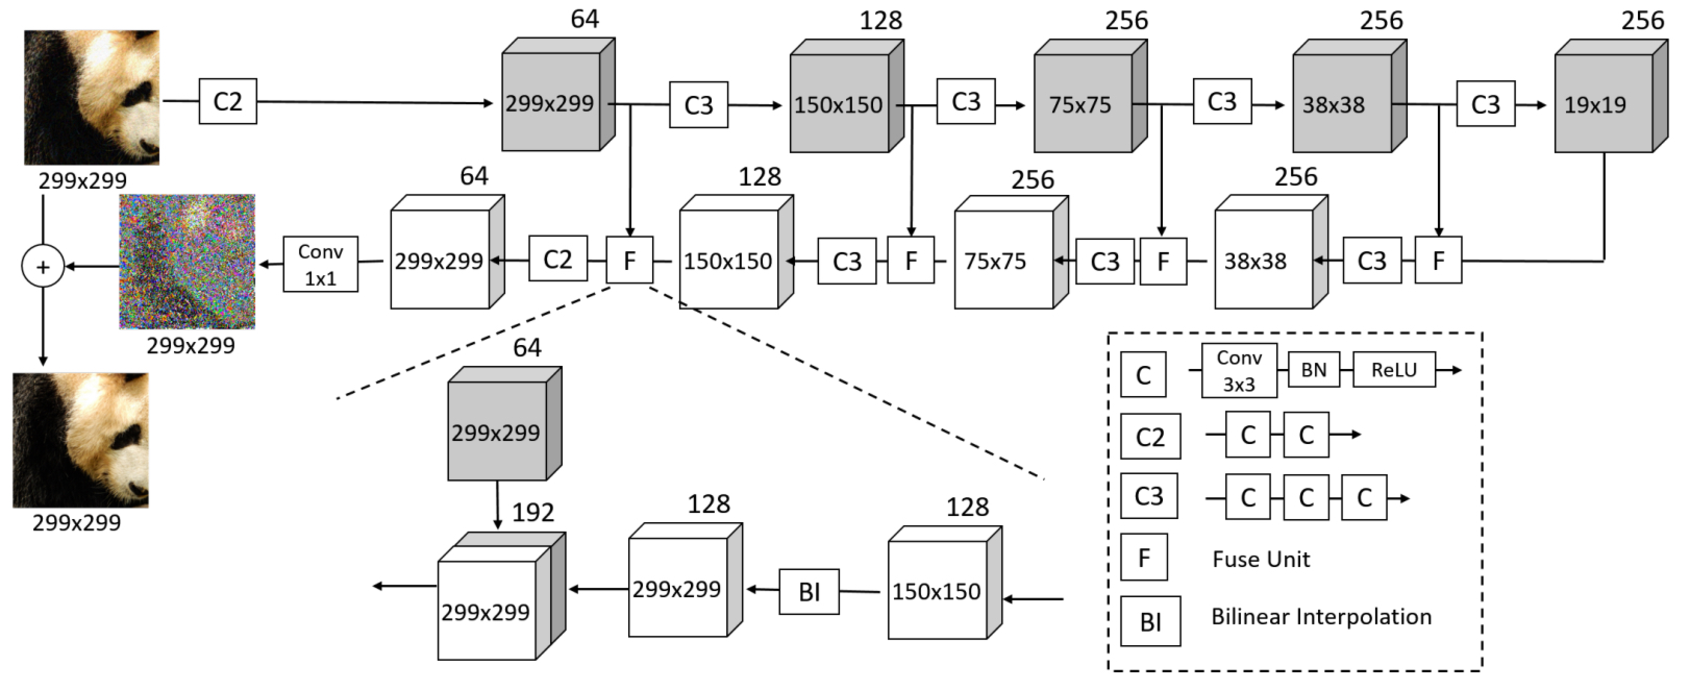
\includegraphics[width=14.0cm]{figures/defense-against-summary.pdf}
\end{center}
\caption{
除去すべき摂動を出力する U-net の概要.
Ck は k 個 convolution を繰り返すという記法で, 右方向は $3 \times 3$ の convolution で 1 つ目は $2 \times 2$ の stride でそれ以外は $1 \times 1$ であり, 左方向は $1 \times 1$ の convolution で stride は $1 \times 1$ である.
Fuse Unit の部分で各スケールで connection を張っているのが U-net の特徴である.
図は \cite{liao2018defense} より引用.}
\label{fig:defense-against-summary}
\end{figure}

基本戦略は外部リソース利用で, 入力データから摂動を除去する U-net を使うため, それを準備する人的コストが必要で推論速度への影響も大きい.

構造は差し引くべき摂動を作成する U-net ということで定まっているので, 残る問題はどんな loss function で学習するかである.
ナイーブな loss function としては単純なピクセル単位の $l_1$ loss が考えられる.
元の入力データ $x$ から始めて, 何かしらの攻撃手法で adversarial examples を用いて $x_{\text{adv}}$ を準備する.
これを U-net に入力すると $- \omega$ が出力されるため, $|x - (x_{\text{adv}} - \omega)|$ を loss とするというものである.
この loss function でも一定の効果が出ることが示されているが, 予測モデルの高次特徴量を使うことでより良い結果が得られることが実験で示されている.
これは具体的には図 \ref{fig:defense-against-three-types} のようになっており, loss に使う出力の層が異なる程度で大きな違いはない.
%
\begin{figure}[htbp]
\begin{center}
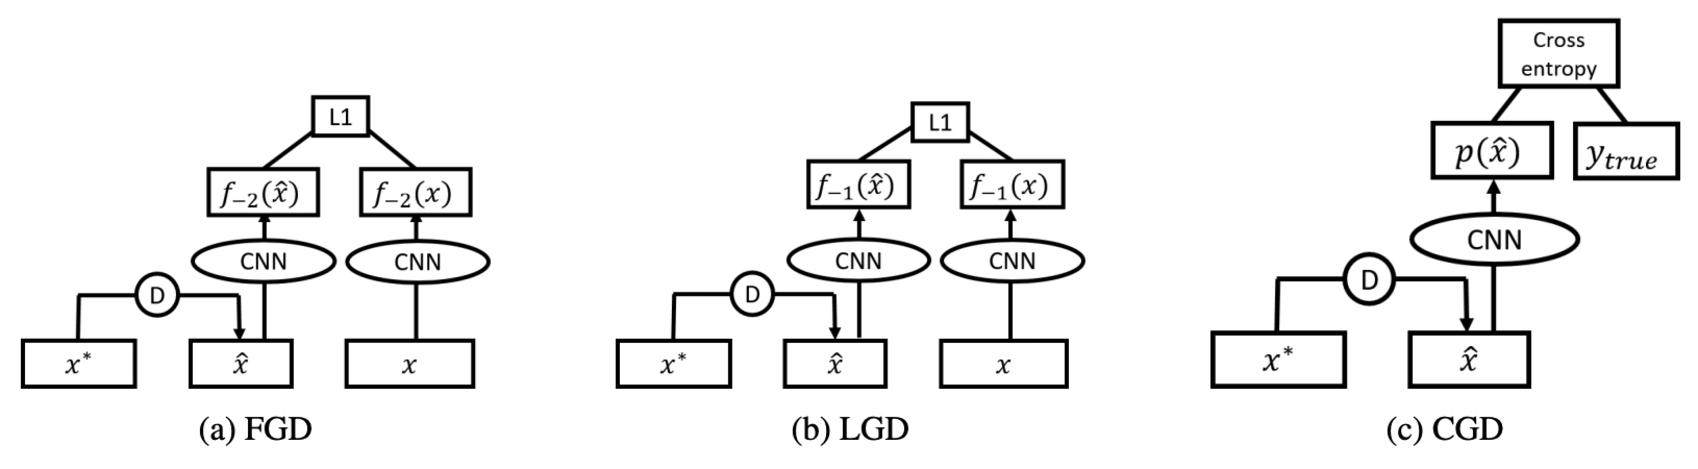
\includegraphics[width=14.0cm]{figures/defense-against-three-types.pdf}
\end{center}
\caption{
予測モデルの高次特徴量を使った loss function 構成のパターン.
$x^*$ は $x_{\text{adv}}$ に対応し, $f_{-l}$ は $-1$ が logit で $-2$ がその前の層の出力を意味する.
D は denoiser で U-net で生成した摂動を用いて clean データを作成するもの.
それぞれ予測モデルの異なる層の出力を用いて loss を構成している.
図は \cite{liao2018defense} より引用.
}
\label{fig:defense-against-three-types}
\end{figure}
%

データは ILSVRC2012 で予測モデルとしては pre-trained inception-v3 を用いる.
U-net は学習にもテストにも adversarial examples が必要となるため, 図 \ref{fig:defense-against-make-adv-examples} のように作成している.
様々なパターンを準備しているが, 学習用の adversarial examples としては予測モデルに近しいタイプのモデルで攻撃手法のパラメタを変えながら作成しており, テストとして同じモデル構造から作成したものと似たモデル構造から作成したもの, となっている.
%
\begin{figure}[htbp]
\begin{center}
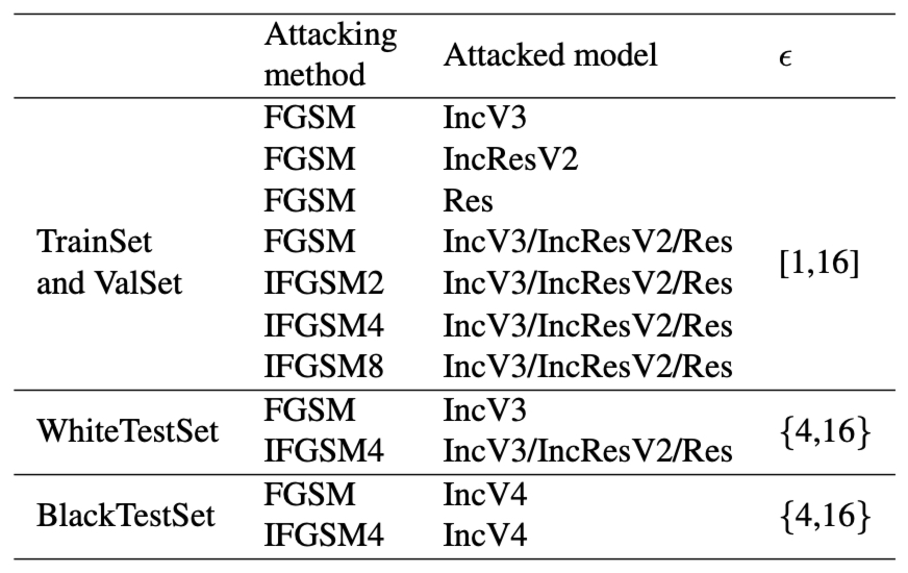
\includegraphics[width=10.0cm]{figures/defense-against-make-adv-examples.pdf}
\end{center}
\caption{
学習とテスト用の adversarial examples の作成方法.
攻撃手法としては FGSM もしくは I+FGSM を用いており, モデルは Inception (Inc), IncRes (InceptionResnet), Res (ResNet50-v2), を用いている.
$\epsilon$ は摂動の大きさで, [1, 16] は 1/255 から 16/255 の間のランダムにサンプルした値を adversarial examples を作るのに使っており, \{4, 16\} は 4/255, 16/255 の 2 つの値それぞれを使っている.
WhiteTestSet は予測モデルと同じモデル構造を使っているという意味で, BlackTestSet は予測モデルと異なるモデル構造を使っているという意味である.
学習と検証に 210,000 枚と 70,000 枚を準備し, テストは WhiteTestSet と BlackTestSet それぞれ 40,000 枚準備する.
図は \cite{liao2018defense} より引用.
}
\label{fig:defense-against-make-adv-examples}
\end{figure}

実験結果が図 \ref{fig:defense-against-result-table} となる.
提案手法は clean データに対する degradation が発生しているがその程度はそれほど著しくはない.
入力画像空間で loss を構成する PGD は WhiteTestSet での性能が低いが, 高次特徴を用いた下三行の手法は WhiteTestSet に対する精度も高く保てている.
ただし, U-net の存在は攻撃者には知られていないという問題設定である.
%
\begin{figure}[htbp]
\begin{center}
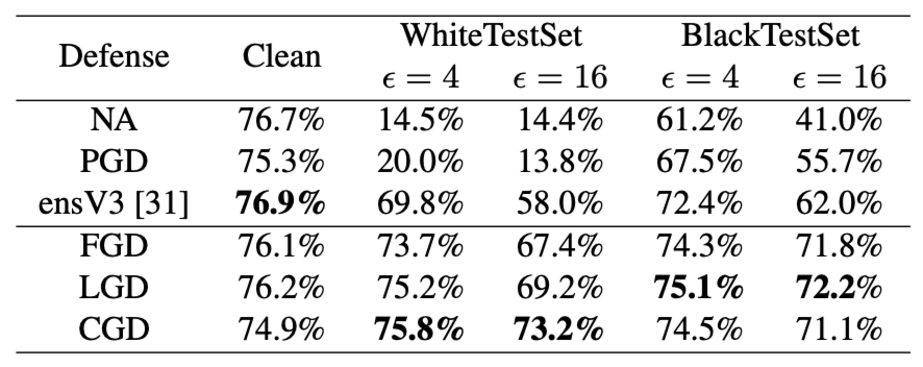
\includegraphics[width=10.0cm]{figures/defense-against-result-table.pdf}
\end{center}
\caption{
テストデータに対する精度を調べた結果.
PGD は $|x - (x_{\text{adv}} - \omega)|$ を loss とするモデルで, envV3 は \cite{tramer2017ensemble} のモデルで, 下三行は図 \ref{fig:defense-against-three-types} で定義したものである.
図は \cite{liao2018defense} より引用.
}
\label{fig:defense-against-result-table}
\end{figure}
%

この手法は adversarial examples に対して正しい予測をするために, 入力データ自体を clean なものに差し替えるのではなく除去すべき摂動に注目してそれを出力する U-net を作成したという着眼点がユニークである.
また, adversarial examples の実験では MNIST や CIFAR などのサイズも数も小さなデータセットで実施することも多いが, 大きめのデータセットで実験をしているのも良い点である.
ただし, 攻撃者が denoiser の存在を知らないという設定でのみ結果を調べていることは注意が必要である.



\subsection{Thermometer Encoding: One Hot Way To Resist Adversarial Examples}
\label{subsec:thermometer-encoding}
%
\begin{table}[htbp]
\begin{center}
\begin{tabular}{|c|c|}
\hline
分類の観点 & この手法が該当するもの \\
\hline
基本戦略 & 入力データ変更 \\
使用する外部リソース & 必要なし \\
対応コスト & 人的コスト:中, 推論コスト:中 \\
\hline
\multicolumn{2}{|c|}{非公式実装: \href{https://github.com/IBM/adversarial-robustness-toolbox/tree/master/art/defences}{https://github.com/IBM/adversarial-robustness-toolbox/tree/master/art/defences}} \\
\hline
\end{tabular}
\label{tb:thermometer_encoding_summary}
\end{center}
\end{table}
%

これは \cite{buckman2018thermometer} によって提案された手法であり,  相対的な距離情報を保つ非線形な離散化で離散化した入力を扱うモデルを学習して防御する.

基本戦略は入力データ変更で外部リソースも必要としないが, 入力データをカテゴリカル変数に置き換えるため, 予測モデルをそれに合わせて学習しておく必要がある.

\cite{goodfellow2014explaining} で指摘された DNN が adversarial examples に対して線形モデルのように振舞うという性質は, 非線形性を持ち込む activation function が ReLU など線形に近いものを用いているためだと考えられる.
とはいえ, それを防ぐために非線形な関数を使おうと例えば RBF を使うと, 学習が難しくなってしまう.
この論文では入力を離散化することで非線形性を導入して adversarial examples に対する防御とする.
ここでの離散化は重みを 32 bit から 8 bit にするというタイプのものではなく, 入力の各ピクセルを量子化して 4 個のカテゴリカル変数にして扱う.
そのため, 離散化の有無で入力の shape が異なる別のモデルであり, 一から学習しなければならない.

入力の離散化手順を見ていく.
まず, $\theta \in [0, 1]$ の実数を等間隔に量子化する $b (\theta)$ を定義する.
これは $0 < b_1 < b_2 < \dots < b_k = 1$ として $\theta \leq b_\alpha$ なる最大のインデックス $\alpha \in \{1, \dots, k\}$ を返す関数である.
入力データの各ピクセルをこの関数で量子化し, そこからカテゴリカル変数に置き換える encoding 手法として二つの手法を考える.

一つ目は one-hot encoding $d_{\text{one-hot}}: x_i \rightarrow \{0, 1\}^k$ で, 以下のように定義される.
%
\begin{eqnarray}
d_{\text{one-hot}} (x_i) &=& \chi (b(x_i))\\
\chi (j)_i &=& \left\{ \begin{array}{l}
1 \ \ \text{if} \ l = j \\
0 \ \ \text{otherwise.} \\
\end{array} \right.
\label{eq:thermometer-encoding-onehot}
\end{eqnarray}
%
これは単純な手法であるが, どんな入力に対しても $\|\chi (b(x_i))\|_2  = \|\chi (b(x_j))\|_2 = 1 \ (b(x_i) \neq b(x_j))$ となるため, $x_i, x_j$ の順序情報を潰してしまう.
離散化したときに同じ範囲に属するものは異なる範囲に属するものよりも似ていると考えるのが自然だが, ここでの離散化はそうなっておらず好ましくない.

これを解決するために考案した二つ目の手法が thermometer encoding $d_{\text{thermometer}}: x_i \rightarrow \{0, 1\}^k$ で, 以下のように定義される.
%
\begin{eqnarray}
d_{\text{thermometer}} (x_i) &=& \tau (b(x_i))\\
\tau (j)_i &=& \left\{ \begin{array}{l}
1 \ \ \text{if} \ l \geq j \\
0 \ \ \text{otherwise.} \\
\end{array} \right.
\label{eq:thermometer-encoding-thermometer}
\end{eqnarray}
%
こちらの場合, $b(x_i) \neq b(x_j)$ かつ $x_i < x_j$ なる $i,j$ に対して $\|\tau(b(x_i))\|_2 < \|\tau(b(x_j))\|_2$ が成り立つためより目的に適った離散化である.

上記二つの離散化の例は図 \ref{fig:termometer-encoding-encodings} の通りである(k = 4 の場合).
各ピクセルの値がそれぞれの encoding によって 5 個の要素からなるカテゴリカル変数に変換される様子が見て取れる.
%
\begin{figure}[htbp]
\begin{center}
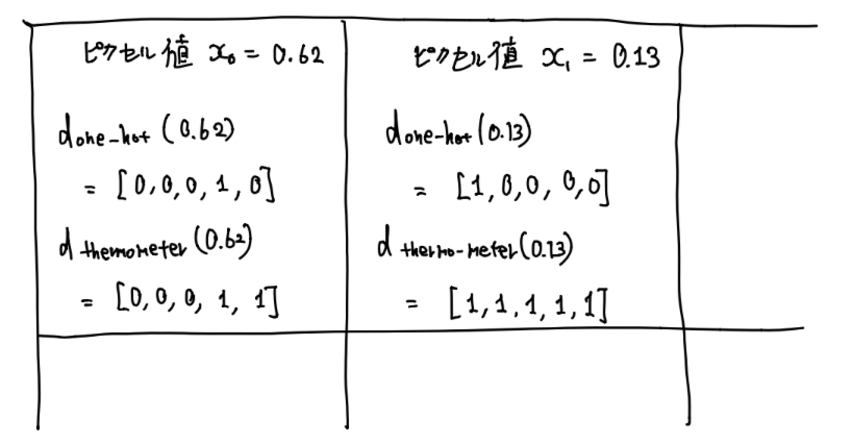
\includegraphics[width=10.0cm]{figures/termometer-encoding-encodings.pdf}
\end{center}
\caption{
one-hot encoding と thermometer encoding の $k=4$ の例.
図は \cite{buckman2018thermometer} より引用.
}
\label{fig:termometer-encoding-encodings}
\end{figure}

離散化操作によって微分不可能になるため, このモデルに対して adversarial examples を作成するための手法が必要となる.
以降の話は thermometer encoding を対象とするが, encoding を置き換えればそのまま one-hot encoding にも適用できる.
ここでの $x^{(t)}_{\text{adv},i}$ は $x_i$ のピクセル値を離散化して $k$ 次元のベクトルとした $\tau(b(x_i))$ に加える摂動の $t$ 回目のステップでの $k$ 次元のベクトルとして扱う.
%
\begin{eqnarray}
x^{(0)}_{\text{adv},i} &=& d_{\text{thermometer}} (x_i + U(-\epsilon, \epsilon)).\\
\text{harm} (x^{(t)}_{\text{adv},i})_l &=& \left\{ \begin{array}{l}
(x^{(t)}_{\text{adv},i} - \tau (l))^T \cdot \frac{\partial J}{\partial x^{(t)}_{\text{adv},i}} \ \ \text{if} \ ^{\exists}(\epsilon \leq \eta \leq \epsilon) \ \text{s.t.} \ b(x_i + \eta) = l. \\
0 \ \ \text{otherwise.} \\
\end{array} \right.\\
x^{(t+1)}_{\text{adv},i} &=& \tau \left(\argmax \left[ \text{harm} (x^{(t)}_{\text{adv},i}) \right]\right).
\label{eq:thermometer-encoding-dga}
\end{eqnarray}
%
まず, 元の入力に一様乱数からサンプルしたランダムなノイズを加える.
次に量子化の各範囲に対して, 元の入力に対して摂動を加えることでその範囲に属することができる場合のみ, 離散化した $x_{\text{adv},i}$ の微分で loss が大きくなる方向を見つけて, 現状から $\tau(l)$ に変わった場合の loss の増大分を計算する.
どの $\tau(l)$ に変えるのが最も loss を増大させるかを比べてアップデートする.
最初に与えるランダムなノイズの影響力が大きいため, 実際には複数回走らせて良い結果を採用する.

途中の状態を softmax を用いて連続量にするという Logit-Space Projected Gradient Ascent (LS-PGA) という手法も提案している.
これは連続量にした $u$ と温度パラメタ $T$ を用いて以下のように adversarial examples を定める.
%
\begin{eqnarray}
x^{(t)}_{\text{adv},i} &=& \mathbb{C} \left( \text{softmax} \left( \frac{u^{(t)}_i}{T^{(t)}} \right) \right) \ \ \text{where} \ \ \mathbb{C}(c)_l = \sum_{j = 0}^l c_l. \\
x^{(\text{final})}_{\text{adv},i} &=& \tau \left( \argmax \left[ u^{(\text{final})}_i \right] \right).\\
T^{(t)} &=& T^{(t - 1)} \cdot \delta.
\label{eq:thermometer-encoding-lspga}
\end{eqnarray}
%
連続量にした $u^{(t)}_i$ は以下のようにステップサイズ $\xi$ で更新していく.
%
\begin{eqnarray}
u^{(0)}_i &=& \left\{ \begin{array}{l}
\mathcal{N} (\mathbf{0}, \mathbf{1}) \ \ \text{if} \ ^{\exists}(\epsilon \leq \eta \leq \epsilon) \ \text{s.t.} \ b(x_i + \eta) = l. \\
- \infty \ \ \text{otherwise.} \\
\end{array} \right.\\
(u^{(t + 1)}_i)_l &=& \left\{ \begin{array}{l}
(u^{(t)}_i)_l + \xi \cdot \text{sign} \left( \frac{\partial L}{\partial u^{(t)}_i} \right)_l \ \ \text{if} \ ^{\exists}(\epsilon \leq \eta \leq \epsilon) \ \text{s.t.} \ b(x_i + \eta) = l. \\
- \infty \ \ \text{otherwise.} \\
\end{array} \right.
\label{eq:thermometer-encoding-logit}
\end{eqnarray}
%

実験は MNIST, CIFAR, SVHN のデータを用いてモデルは WideResNet を用いている.
MNIST は簡単であまり意味があるものではなく, それ以外は傾向が似ているため, ここでは CIFAR10 の結果だけを載せる.
結果は図 \ref{fig:thermometer-encoding-cifar10} の通りで, 特に adversarial training と組み合わせることで提案手法が FGSM\footnote{
ここの FGSM を離散化したモデルにどう適用しているかは著者にはよく分からない.
離散化していないモデルで adversarial examples を作成してから離散化しているのだろうか.
} に対しても論文で提案した攻撃手法に対しても高い性能を発揮していることが分かる.
%
\begin{figure}[htbp]
\begin{center}
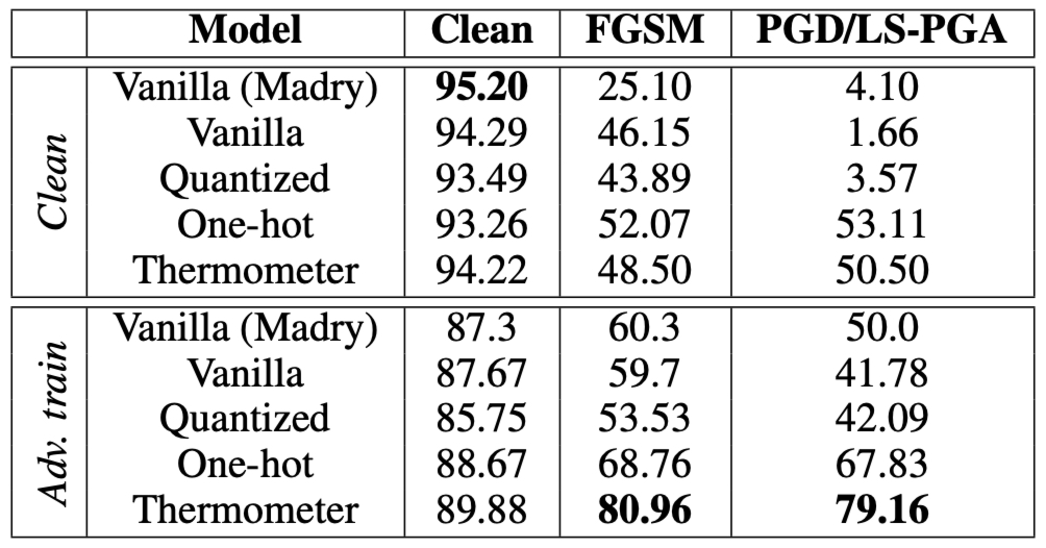
\includegraphics[width=10.0cm]{figures/thermometer-encoding-cifar10.pdf}
\end{center}
\caption{
CIFAR10 の実験結果.
モデルは WideResNet で, Vanilla は \cite{madry2017towards} の結果で括弧付きが論文の結果で括弧なしがその再現実装の結果.
図は \cite{buckman2018thermometer} より引用.
}
\label{fig:thermometer-encoding-cifar10}
\end{figure}
%

この手法は入力を離散化するというシンプルな手法で高い性能を発揮した点が興味深く, このようなアイデアは今後も色々と出てくるだろうと期待される.



\subsection{Stochastic Activation Pruning for Robust Adversarial Defense}
\label{subsec:stochastic-activation}
%
\begin{table}[htbp]
\begin{center}
\begin{tabular}{|c|c|}
\hline
分類の観点 & この手法が該当するもの \\
\hline
基本戦略 & 予測モデル変更 \\
使用する外部リソース & 必要なし \\
対応コスト & 人的コスト:小, 推論コスト:中 \\
\hline
\multicolumn{2}{|c|}{公式実装: \href{https://github.com/Guneet-Dhillon/Stochastic-Activation-Pruning}{https://github.com/Guneet-Dhillon/Stochastic-Activation-Pruning}} \\
\hline
\end{tabular}
\label{tb:stochastic-activation-summary}
\end{center}
\end{table}
%

これは \cite{dhillon2018stochastic} によって提案された手法であり, 推測時に各 activation layer の出力をその絶対値の小ささに応じて確率的に 0 にすることで摂動が増幅されて異なる予測になることを防ぐ.
公式実装は公開されているが, 該当機構の部分は MXNet \cite{chen2015mxnet} に含まれており実装ではそれを呼び出しているだけである.

基本戦略は予測モデル変更であり, これは学習済みモデルに導入できるものなので人的コストは低い.
ただし推測時に大量のサンプリングを必要とするので推論コストは小さくない.

アイデアはシンプルで実装も速度を考慮しなければ難しくはない.
実際の手続きはアルゴリズム \ref{alg:adversarial-examples-alg} のようになる.
activation function が出現する毎に, 出力の絶対値の大きさに従う確率で所定の回数サンプリングをして, 選ばれなかった出力を 0 に差し替えていくというものになっている.
多項分布からのサンプリングで一般に同じ index が複数回サンプリングされ得るが, サンプリングされた回数に依らず以降の処理を実施する.
典型的なサンプリング回数は $c \times h \times w$ で元の出力の要素数回であり, これを SAP-100 などと書く.
重複ありのサンプリングなので 100 より大きくすることも可能である.
%
\begin{algorithm}
\caption{Stochastic Activation Pruning のアルゴリズム}
\label{alg:stochastic-activation-alg}
\begin{algorithmic}[1]
    \State Input: 入力データ $x$, 各層の重み行列 $W^{(i)}$, 各層の activation function $\phi^{(i)}$, 各層でのサンプリング回数 $r^{(i)}$.
    \State Output: 最後の activation function の出力 $h^{(n)}$.
    \State 初期化: $h^{(0)} \leftarrow x$.
    \For {各層 $i$}
    \State activation function の出力を計算: $h^{(i)} \leftarrow \phi^{(i)} (W^{(i)} h^{(i - 1)}) $.
    \State 出力の絶対値の大きさに従って確率値に変換: $p_{j}^{(i)} \leftarrow \frac{|h_{j}^{(i)}|}{\sum_j |h_{j}^{(i)}|}$.
    \State 非ゼロの activation function の出力の index を保持する集合を初期化: $S \leftarrow \{\}$.
    \State ループカウンタの初期化: $k \leftarrow 0$.
    \While {$k < r^{(i)}$}.
    \State サンプリング: $s \sim \text{categorical} (p^{(i)})$.
    \State サンプリングされた index を集合に追加: $S \leftarrow S \cup \{s\}$.
    \For {各 $j \not\in S$}
    \State サンプリングされなかったものは 0 にする: $h_{j}^{(i)} \leftarrow 0$.
    \EndFor
    \For {各 $j \in S$}
    \State 出力のスケーリング: $h_{j}^{(i)} \leftarrow \frac{h_{j}^{(i)}}{1 - (1 - p^{(i)}_{j})^{r^{(i)}}}$.
    \EndFor
    \State ループ変数をインクリメント: $k \leftarrow k + 1$.
    \EndWhile
    \EndFor
    \Return $h^{(n)}$
\end{algorithmic} 
\end{algorithm}

単純な dropout との違いは, 出力の絶対値の大きさによってサンプリングされる確率が変わるというものである.
これによって, 学習済みのモデルに導入することができ, 重要な出力は残りやすくなるため元の予測の性能にも悪影響が少ない.
定義から明らかなように, Stochastic Activation Pruning は, サンプリング回数が多ければ元のモデルの予測と近くなり, サンプリング回数が少なければ元のモデルの予測の degradation が起きるが adversarial examples には強くなってくれる.
うまくバランスを取れるようなサンプリング回数を見つけることができれば有用である, というのが論文の主張である.

ただ, 多数のサンプリングを要求するため実用にはほど遠いというのが著者の感想である\footnote{
のちに \ref{sec:exp} 章の実験で述べるように, 実装したものもうまく動かなかった (単に実装がバグっているだけかもしれないが).
}.
論文で表記しているのは FGSM による adversarial examples を作成するのに要する時間であるが, 512 枚の画像に対して 8 GPU で 20 秒程度掛かっていると報告している.

実験はデータとして CIFAR10 を用いてモデルは ResNet-20 を使用している.
adversarial examples は FGSM を用いて作成している.
結果は図 \ref{fig:adversarial-examples-result-table} の通りで, ランダムなノイズに関しては効果は出ていないが adversarial examples に関しては防御なしのモデルと比べて正答率が高くなっている.
モデル内部で確率的処理が含まれているので, 予測モデルと同じ Stochastic Activation Pruning 有りのモデルを使って adversarial examples を作っても正答率が高いというのは特徴的である.
%
\begin{figure}[htbp]
\begin{center}
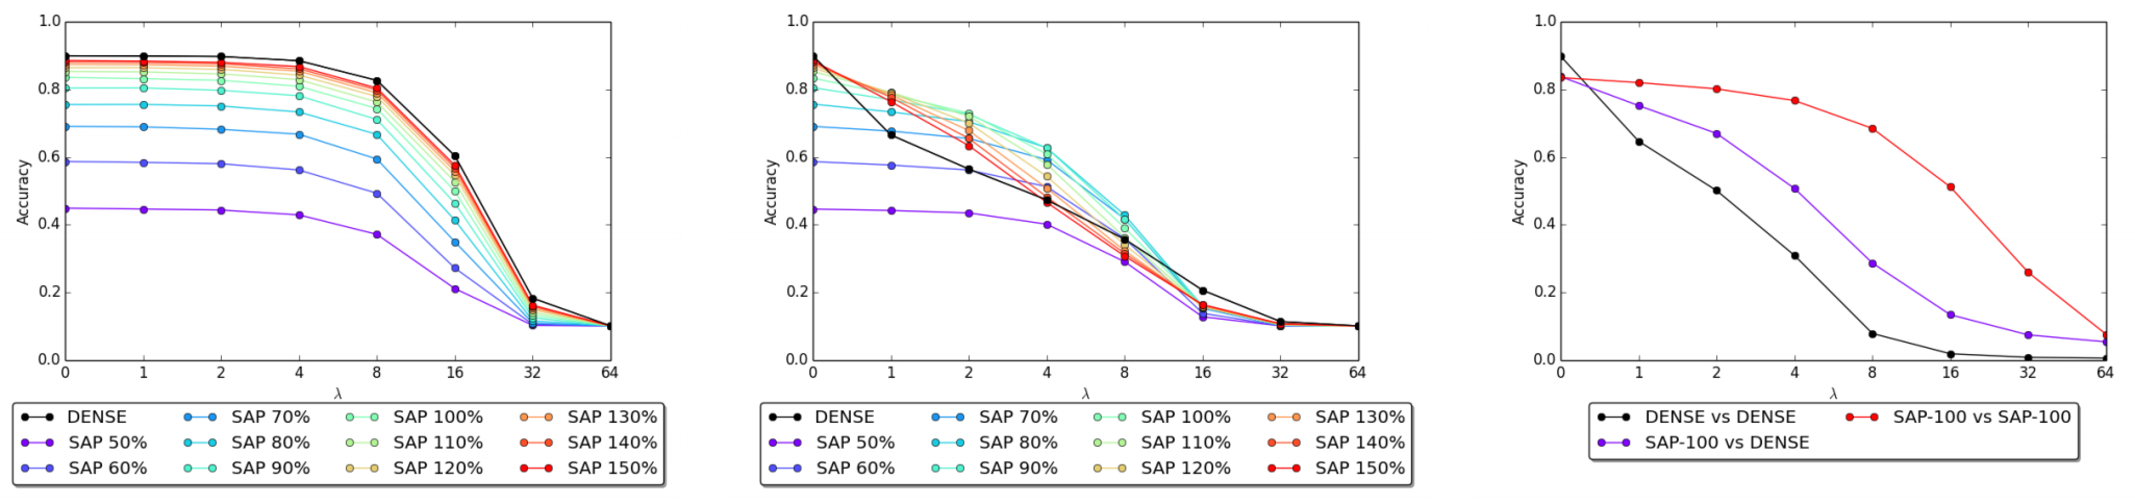
\includegraphics[width=16.0cm]{figures/adversarial-examples-result-table.pdf}
\end{center}
\caption{
CIFAR10 で FGSM で adversarial examples を作成して正答率を測定した結果.
モデルは ResNet-20 を使用.
縦軸は正答率で横軸は FGSM での摂動の大きさの $\epsilon / 255$ の $\epsilon$ である.
左はランダムノイズに対する結果で, 真ん中は FGSM に対する結果で, 右図は (予測モデル) vs (FGSM を作成するのに使用したモデル) の結果である.
図は \cite{dhillon2018stochastic} より引用.
}
\label{fig:adversarial-examples-result-table}
\end{figure}
%

この手法はモデル学習後に導入できる手法でかつ入力データへの操作が必要ないというのが興味深い点である.
確率的な処理により, 予測モデルと同じモデルで adversarial examples を作成しても正答率を高く保てるが, 推論速度への影響が大きく, 実用には向かない.



\subsection{Adversarial Logit Pairing}
\label{subsec:adversarial-logit}
%
\begin{table}[htbp]
\begin{center}
\begin{tabular}{|c|c|}
\hline
分類の観点 & この手法が該当するもの \\
\hline
基本戦略 & 正則化 \\
使用する外部リソース & adversarial examples \\
対応コスト & 人的コスト:中, 推論コスト:小 \\
\hline
\multicolumn{2}{|c|}{公式実装: \href{https://github.com/tensorflow/models/tree/master/research/adversarial_logit_pairing}{https://github.com/tensorflow/models/tree/master/research/adversarial\_logit\_pairing}} \\
\hline
\end{tabular}
\label{tb:adversarial-logit-summary}
\end{center}
\end{table}
%

これは \cite{kannan2018adversarial} によって提案された手法であり, adversarial training 時の loss function にさらに clean データと adversarial examples の logit の $l_2$ loss を加えるものである.
logit 空間において clean データと adversarial examples が同じものになるように正則化を加えることで, adversarial examples に対する予測を正しいものに導こうという戦略である.

分類の観点は adversarial training (\ref{subsec:explaining-and} 節) と同じで, loss function が異なるのみである.

ミニバッチの loss function は以下の通りである.
%
\begin{eqnarray}
\frac{1}{B} \sum_b^B \left( J(f, x^{(b)}, y^{(b)}) + J(f, x^{(b)}_{\text{adv}}, y^{(b)}) \right) + \frac{\lambda}{B} \sum_b^B \| f_{\text{logit}} (x^{(b)}) - f_{\text{logit}} (x^{(b)}_{\text{adv}}) \|_2.
\label{eq:adversarial-logit-loss}
\end{eqnarray}
%
ここで, 第一項と第二項は $J$ として cross entropy を使い, これらは \ref{eq:explaining-and-loss} 式の adversarial training で $\alpha = 0.5$ とした場合と等しく, 論文ではこの部分を mixed-minibatch PGD と呼んでいる.
第三項が logit pairing の項で, 単純な logit の $l_2$ loss である.
パラメタとして $\lambda$ を導入しているが, 実験においては $\lambda = 1$ としてそれ以外の値は試していない.
これが提案手法となるが, clean データだけで同じように logit pairing を導入した clean logit pairing も提案している.
%
\begin{eqnarray}
\frac{1}{B} \sum_b^{B} J(f, x^{(b)}, y^{(b)}) + \frac{\lambda}{B} \sum_b^{B/2} \| f_{\text{logit}} (x^{(b)}) - f_{\text{logit}} (x^{(b + B/2)}_{\text{adv}}) \|_2.
\label{eq:adversarial-logit-clp}
\end{eqnarray}
%
これを gaussian ノイズを使って学習するだけで単純な adversarial training に近いくらいの性能が出せることを示し, 単なるベースライン以上に面白い結果だが論文では述べられている(本書ではこの手法に関する結果は省略する).

実験は MNIST と SVHN データに対してはモデルは LeNet \cite{lecun1998gradient}, ILSVRC2012 データに対しては inception-v3 を用いている.
MNIST と SVHN に関してはほぼ同様の結果なので, SVHN の結果のみを載せる.
その結果が図 \ref{fig:adversarial-logit-result-svhn} であり, clean データに対してはやや性能が落ちるが adversarial examples に対する性能は単純な adversarial training よりも向上している.
%
\begin{figure}[htbp]
\begin{center}
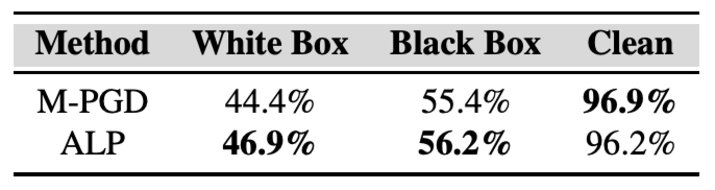
\includegraphics[width=10.0cm]{figures/adversarial-logit-result-svhn.pdf}
\end{center}
\caption{
SVHN データで LeNet を用いて I+FGSM で作成した adversarial examples に対する正答率を調べた結果.
M-PGD は I+FGSM で作成した adversarial examples で adversarial training をしたモデルで, ALP が提案手法で学習したモデルである.
図は \cite{kannan2018adversarial} より引用.
}
\label{fig:adversarial-logit-result-svhn}
\end{figure}
%

ILSVRC2012 の結果が図 \ref{fig:adversarial-logit-result-imagenet} である.
ILSVRC2012 はクラス数が多くて難しい予測となるため, 従来手法では adversarial training をしても正答率がほとんど上がらないという問題があったが, 提案手法では明確に正答率が向上している.
%
\begin{figure}[htbp]
\begin{center}
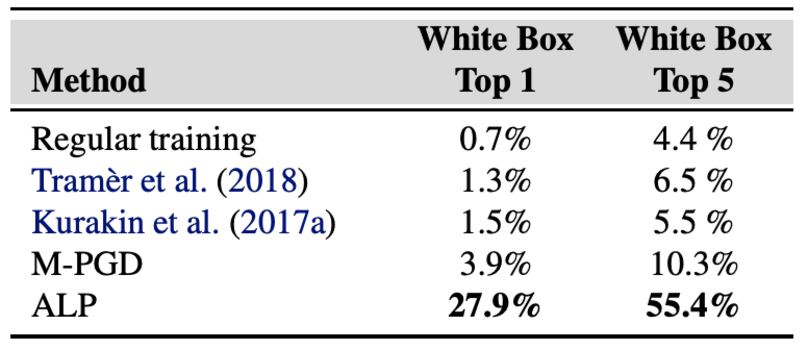
\includegraphics[width=10.0cm]{figures/adversarial-logit-result-imagenet.pdf}
\end{center}
\caption{
ILSVRC2012 データで inception-v3 を用いて I+FGSM で作成した adversarial examples に対する正答率を調べた結果.
Tramer et a.l (2018) は \cite{tramer2017ensemble} の ensemble adversarial training で学習したモデルで, Kurakin et al. (2017a) は \cite{kurakin2016adversarial} の adversarial training で学習したモデルである.
M-PGD は I+FGSM で作成した adversarial examples で adversarial training をしたモデルで, ALP が提案手法で学習したモデルである.
図は \cite{kannan2018adversarial} より引用.
}
\label{fig:adversarial-logit-result-imagenet}
\end{figure}
%

この手法は正則化として logit pairing を導入した点が興味深く, これまでの予測クラス部分のみに注目している adversarial training よりも, モデルが adversarial examples を clean データのように扱う傾向が強くなる.
この手法の登場以降, loss function に様々なアイデアを入れたものが数多く報告されるようになった.



\subsection{Defense-GAN: Protecting Classifiers Against Adversarial Attacks Using Generative Models}
\label{subsec:defense-gan}
%
\begin{table}[htbp]
\begin{center}
\begin{tabular}{|c|c|}
\hline
分類の観点 & この手法が該当するもの \\
\hline
基本戦略 & 入力データ変更 \\
使用する外部リソース & GAN \\
対応コスト & 人的コスト:中, 推論コスト:大 \\
\hline
\multicolumn{2}{|c|}{公式実装: \href{https://github.com/kabkabm/defensegan}{https://github.com/kabkabm/defensegan}} \\
\hline
\end{tabular}
\label{tb:defense-gan-summary}
\end{center}
\end{table}
%

これは \cite{samangouei2018defense} によって提案された手法であり, 図 \ref{fig:defense-gan-architecture} のように clean データで学習した GAN を導入し, 複数乱数から生成した画像から元の入力データに近いものを作成し, それを摂動のない入力とすることで正しい予測をする.
%
\begin{figure}[htbp]
\begin{center}
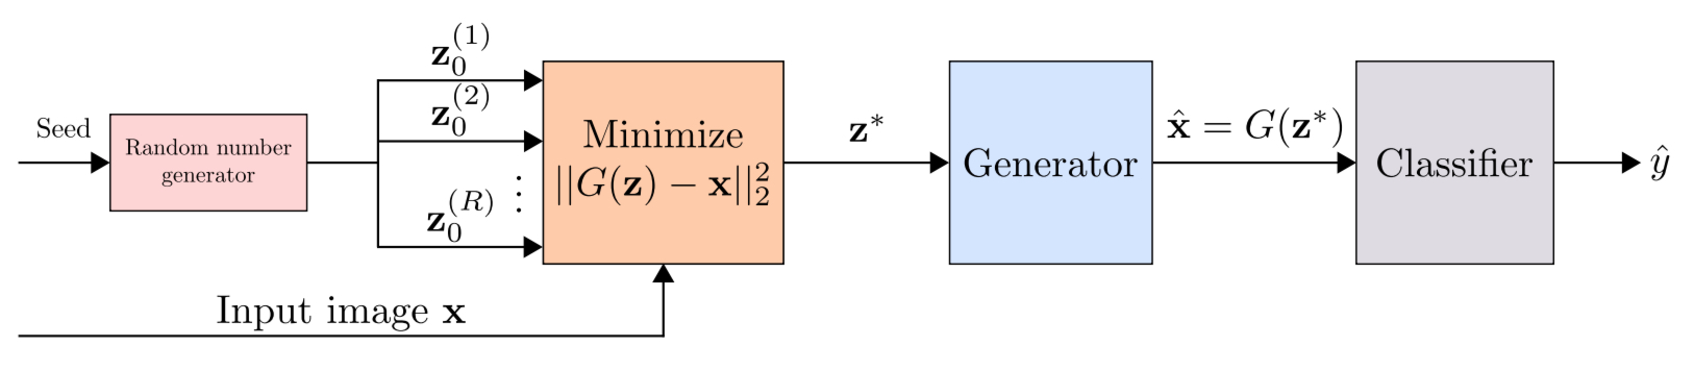
\includegraphics[width=14.0cm]{figures/defense-gan-architecture.pdf}
\end{center}
\caption{
defense-gan のアーキテクチャ.
Minimize のステップで元の入力画像に近い画像を生成する $z^*$ を作成し, それを Generator に入れて画像を生成して予測モデルの入力としている.
図は \cite{samangouei2018defense} より引用.
}
\label{fig:defense-gan-architecture}
\end{figure}
%

この手法は入力する画像を生成モデルを使って生成するという戦略を採用しており, \ref{subsec:generating-natual} 節で見た攻撃手法の防御版とも言える手法である.
予測モデルへの入力画像を生成するためコストは大きい.

この手法では GAN の枠組みで学習した generator と discriminator のうち, generator のみが必要であり, GAN の学習としては安定性の高い WGAN \cite{arjovsky2017wasserstein} の枠組みを使っている.
%
\begin{eqnarray}
\min_G \max_D V_{W} (D, G) = \mathbb{E}_{x \sim p_{\text{data}} (x)} \left[ D(x) \right] - \mathbb{E}_{z \sim p_{z} (z)} \left[ D(G(z)) \right].
\label{eq:defense-gan-wgan}
\end{eqnarray}
%

clean データで学習済みの generator があれば, あとはいかにして元の入力に近い画像を生成するための $z^*$ を作成するかのみが焦点となる.
この論文では, まず初期として $R$ 個の乱数 $z_0^{(i)} (i = 1, \dots, R)$ を準備し, それらを別個に $\| G(z) - x \|_2$ を最小化するように更新して, その中から最も $x$ に近いものを選ぶという戦略を採用している.
問題となるのは $\| G(z) - x \|_2$ の最小化で, これは一般に非凸最適化であるので, 簡単化して $L$ 回の gradient descent で代用している.
これを概念的に示したものが図 \ref{fig:defense-gan-z-optimization} である.
%
\begin{figure}[htbp]
\begin{center}
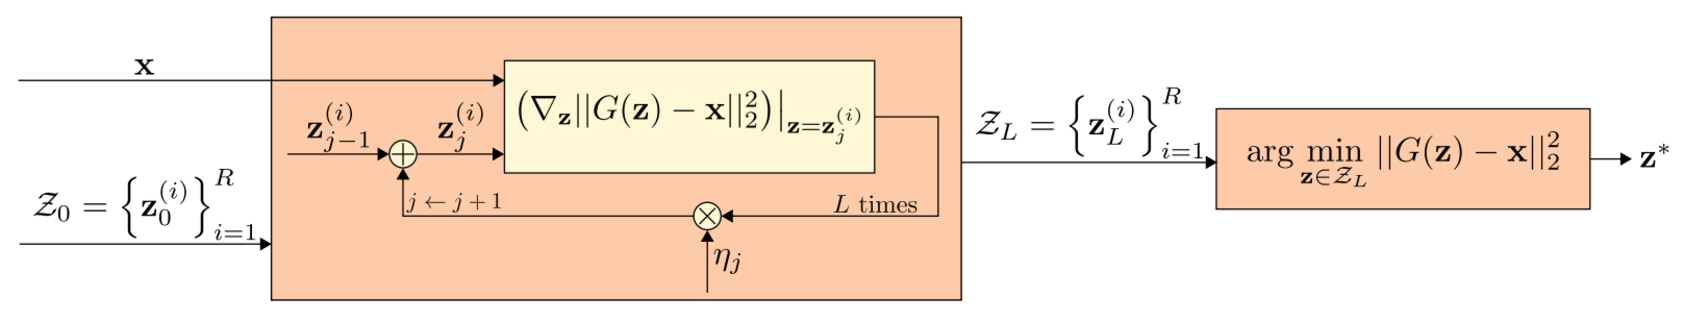
\includegraphics[width=14.0cm]{figures/defense-gan-z-optimization.pdf}
\end{center}
\caption{
元の入力に近い画像を生成する $z$ を作成するための手順.
初期値として $R$ 個の乱数を準備し, それぞれ $L$ 回の gradient descent で更新し, その中から最も入力画像に近い画像を生成する $z$ を $z^*$ として選ぶ.
図は \cite{samangouei2018defense} より引用.
}
\label{fig:defense-gan-z-optimization}
\end{figure}
%
ポイントとなるのは $L$ 回のループ処理で, 攻撃側はこのループ処理を逆に辿って adversarial examples を作成しなければならないので, 特に white box attack に関しては高い性能が期待できる.
一方で防御側にとっても一つの予測に要する時間が長くなるということでもあるので, 一長一短である.

実験は典型的な convolution や ReLU などの 典型的な building block から構成した A $\sim$ E の 5 つのモデルを用いて, データは MNIST と Fashion MNIST を用いている.
傾向に違いはないため Fashion MNIST の結果のみを載せる.
black box attack に対する結果が図 \ref{fig:defense-gan-result-black-box} で white box attack に対する結果が図 \ref{fig:defense-gan-result-white-box} となる.
black box attack に対しては提案手法は adversarial training に負けている結果も多くそこまでインパクトがないが, white box attack に関しては圧勝している.
特に CW は他のモデルでは正答率が総じて低いが, 構造上の利点により提案手法では高い正答率を保っている.
%
\begin{figure}[htbp]
\begin{center}
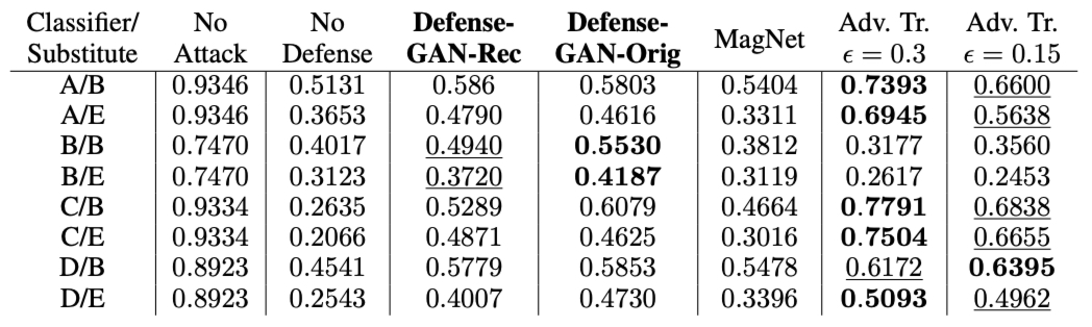
\includegraphics[width=12.0cm]{figures/defense-gan-result-black-box.pdf}
\end{center}
\caption{
Fashion MNIST を用いた black box attack の結果.
Classifier が予測モデルで Substitute が FGSM を使って adversarial examples を作成したモデルを表す.
Defense-GAN-Rec は $G(z^*)$ を使って学習したモデルで Defense-GAN-Orig は $x$ を使って学習したモデルとなる.
図は \cite{samangouei2018defense} より引用.
}
\label{fig:defense-gan-result-black-box}
\end{figure}
%
%
\begin{figure}[htbp]
\begin{center}
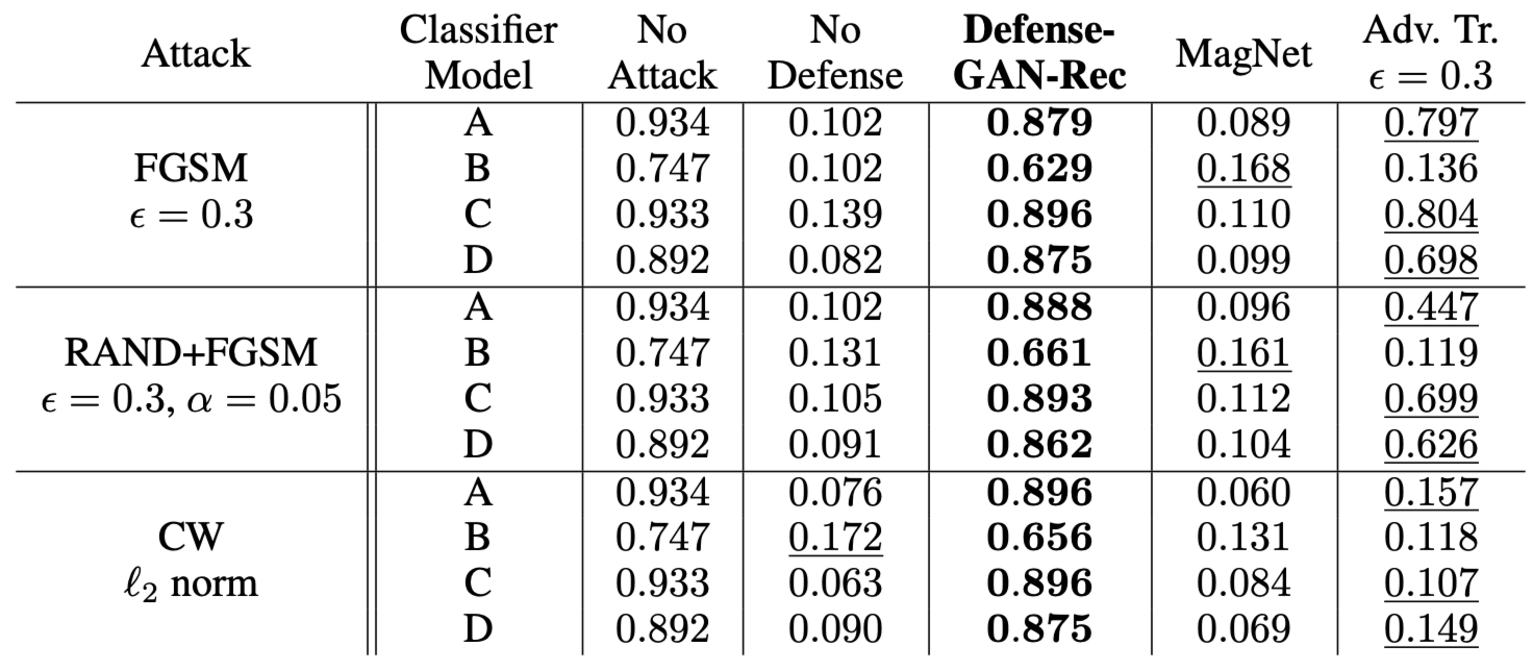
\includegraphics[width=12.0cm]{figures/defense-gan-result-white-box.pdf}
\end{center}
\caption{
Fashion MNIST を用いた white box attack の結果.
Defense-GAN-Rec は $G(z^*)$ を使って学習したモデルを表す.
図は \cite{samangouei2018defense} より引用.
}
\label{fig:defense-gan-result-white-box}
\end{figure}
%

この手法は入力画像そのものを生成するという方向性で摂動の影響が出ないようにしている点が興味深い.
サンプリングや入力画像生成に繰り返しの手順が含まれており, 構造上 white box attack に強い手法になっている.
一方で推論時の速度は著しく低下するため, 一長一短という面も否めない.



\subsection{Feature Denoising for Improving Adversarial Robustness}
\label{subsec:feature-denoising}
%
\begin{table}[htbp]
\begin{center}
\begin{tabular}{|c|c|}
\hline
分類の観点 & この手法が該当するもの \\
\hline
基本戦略 & 予測モデル変更 \\
使用する外部リソース & 必要なし \\
対応コスト & 人的コスト:大, 推論コスト:小 \\
\hline
\multicolumn{2}{|c|}{公式実装: \href{https://github.com/facebookresearch/ImageNet-Adversarial-Training}{https://github.com/facebookresearch/ImageNet-Adversarial-Training}} \\
\hline
\end{tabular}
\label{tb:feature-denoising-summary}
\end{center}
\end{table}
%

これは \cite{xie2019feature} によって提案された手法であり, 非局所的な重み付き和などの denoising block をモデルに取り入れて adversarial training と併用することで摂動の効果を軽減して防御する.
clean データにおける特徴量は空間的に局在しているが adversarial examples における特徴量は広がっているという傾向があるため, 空間的に近いものでなければ値が小さくなるような構造を導入するという戦略である.

この手法の特徴は adversarial examples の feature map の観測に基づいて, モデルに新しい building block を導入している点にある.
図 \ref{fig:feature-denoising-feature-map} が典型的な結果の例で, adversarial examples の feature map は認識したい対象物以外の領域でも大きな値を示しているが, それが提案手法によって抑えられて対象物近辺だけの特徴量が重視されるようになっている. 
%
\begin{figure}[htbp]
\begin{center}
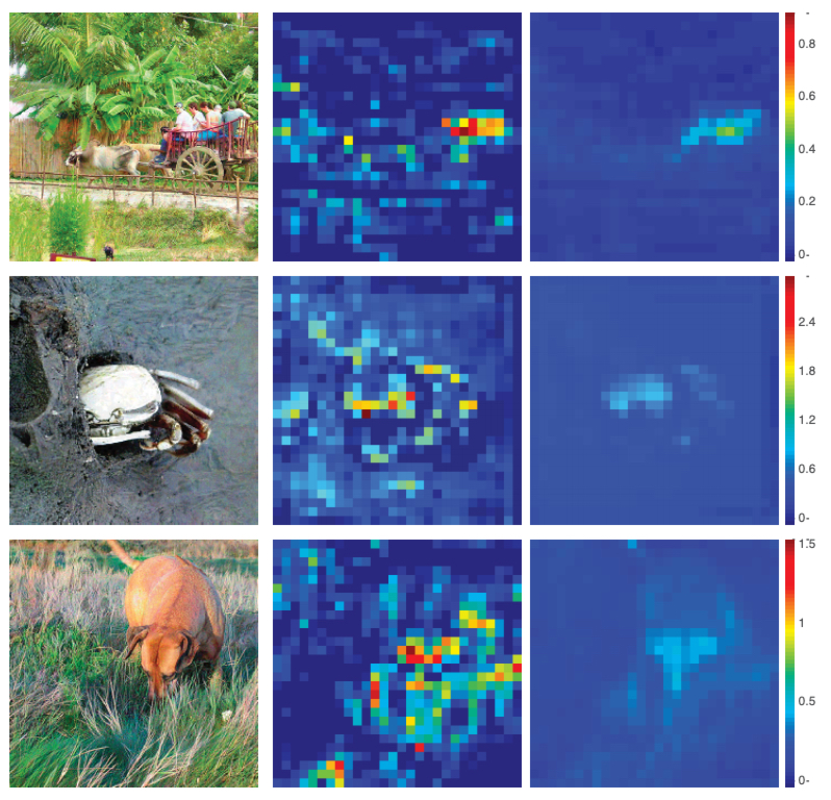
\includegraphics[width=10.0cm]{figures/feature-denoising-feature-map.pdf}
\end{center}
\caption{
adversarial examples の feature map の例.
左列が adversarial examples, 中央列が ResNet-50 の $\text{res}_3$ ブロックのあるチャンネルの feature map で, 右列が同じ feature map の提案手法で denoise した結果である.
図は \cite{xie2019feature} より引用.
}
\label{fig:feature-denoising-feature-map}
\end{figure}
%

この論文では, denoising 操作として非局所重み付き和を導入している.
%
\begin{eqnarray}
\tilde{x}_i = \frac{1}{N(x)} \sum_{\forall j \in \mathcal{L}} d(x_i, x_j) \cdot x_j.
\label{eq:feature-denoising-nonlocal-mean}
\end{eqnarray}
%
ここで, $N(x) = \sum_{\forall j \in \mathcal{L}} d(x_i, x_j)$ で, $d$ は feature に依存する重み関数であり, $\mathcal{L}$ は特徴量の全ての空間的配位の集合を表している.
重み関数は, gaussian $d(x_i, x_j) = \exp (\frac{1}{\sqrt{d}} \theta (x_i)^T \phi (x_j)$ で定義し, $\theta, \phi$ は $1 \times 1$ convolution で embed した特徴量を用いる.
この deonising 操作だけでは必ずしも adversarial examples の広く分布している feature map を denoise する方向に働くとは限らないが, adversarial training と併用することで, clean データの局在している feature map を尊重するように学習することが期待できる.
論文ではこれ以外の $\mathcal{L}, N(x), d$ の選択肢が議論されているが, ここで紹介したものが最も性能が高いため, 本書ではここで紹介したもののみを考える. 
denoising 操作は図 \ref{fig:feature-denoising-denoising-block} の青い部分に対応しており, そのあとさらに $1 \times 1$ convolution を適用して元の $x$ に加えている.
%
\begin{figure}[htbp]
\begin{center}
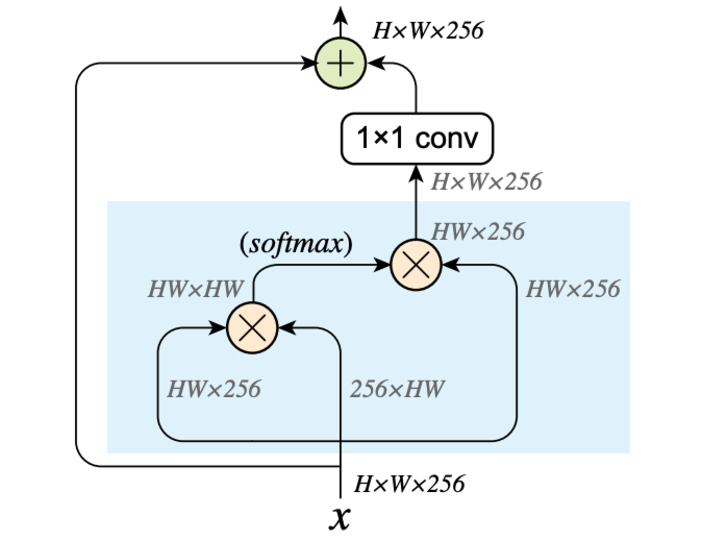
\includegraphics[width=10.0cm]{figures/feature-denoising-denoising-block.pdf}
\end{center}
\caption{
denoising ブロックの全体図.
青い部分が式 \ref{eq:feature-denoising-nonlocal-mean} の denoising 操作に対応している.
図の H,W,256 はそれぞれ Height, Width, チャンネル数を表している.
図は \cite{xie2019feature} より引用.
}
\label{fig:feature-denoising-denoising-block}
\end{figure}
%

実験は ILSVRC2012 データを用いて ResNet モデルで実施している.
adversarial examples は $\epsilon = 16 / 255$ の I+FGMS で作成している.
まず, 先行研究と比べると denoising なしでもかなり性能が高い.
これは モデルアーキテクチャの違いや adversarial training のパラメタの違いに依るものである.
denoising ありの場合は絶対値で 3\% 程度正答率が向上しており, 導入した denoising ブロックの有効性が示されている.
clean データに対する性能は, 同じ構造で adversarial training なしの場合は 79.08\% であるが, ありの場合は 65.30\% であり, degradation が小さくない.
これが主たる結果であるが, 論文では I+FGSM のステップ数を 2,000 回まで変えて結果を調べたり, denoising ブロックの様々な亜種でも実験をしていて, adversarial examples の実験としては大規模なものになっている.
%
\begin{figure}[htbp]
\begin{center}
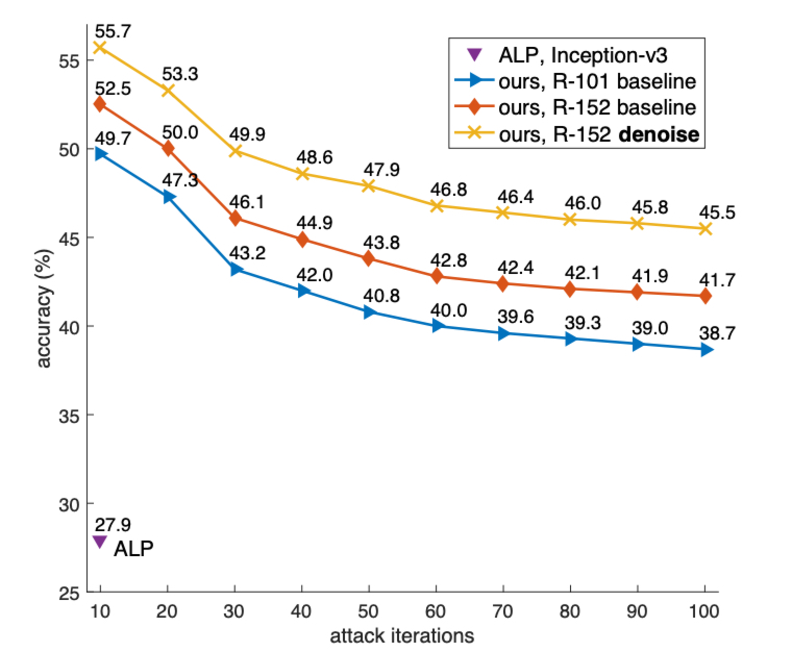
\includegraphics[width=10.0cm]{figures/feature-denoising-result-graph.pdf}
\end{center}
\caption{
ILSVRC2012 の 50,000 枚の validation データで I+FGSM で adversarial examples を作成した正答率を測定した結果.
縦軸が正答率で横軸が I+FGSM のステップ数.
denoising block は 4 つ導入している.
ALP は \ref{subsec:adversarial-logit} 節で紹介した Adversarial Logit Pairing である.
図は \cite{xie2019feature} より引用.
}
\label{fig:feature-denoising-result-graph}
\end{figure}
%

この手法は, モデルの building block として denoising 操作を含む機構を導入して一つのモデルとして学習したという点が興味深い.
入力画像の違いを可視化することは多いが, feature map の可視化と adversarial examples の場合の非局在性を発見し, 導入した機構と adversarial training の組み合わせでそれを取り除いている.



\subsection{Defense Against Adversarial Images using Web-Scale Nearest-Neighbor Search}
\label{subsec:defense-against-adversarial}

\begin{table}[htbp]
\begin{center}
\begin{tabular}{|c|c|}
\hline
分類の観点 & この手法が該当するもの \\
\hline
基本戦略 & 外部リソース使用 \\
使用する外部リソース & 外部データベース \\
対応コスト & 人的コスト:大, 推論コスト:大 \\
\hline
\multicolumn{2}{|c|}{実装なし} \\
\hline
\end{tabular}
\label{tb:defense-against-adversarial-summary}
\end{center}
\end{table}

これは \cite{dubey2019defense} によって提案された手法であり, 図 \ref{fig:defense-against-adversarial-summary} のように, 入力に近い画像を外部データベースから kNN で取得し, それぞれの softmax 値を重み付き平均を取って予測する手法である.
%
\begin{figure}[htbp]
\begin{center}
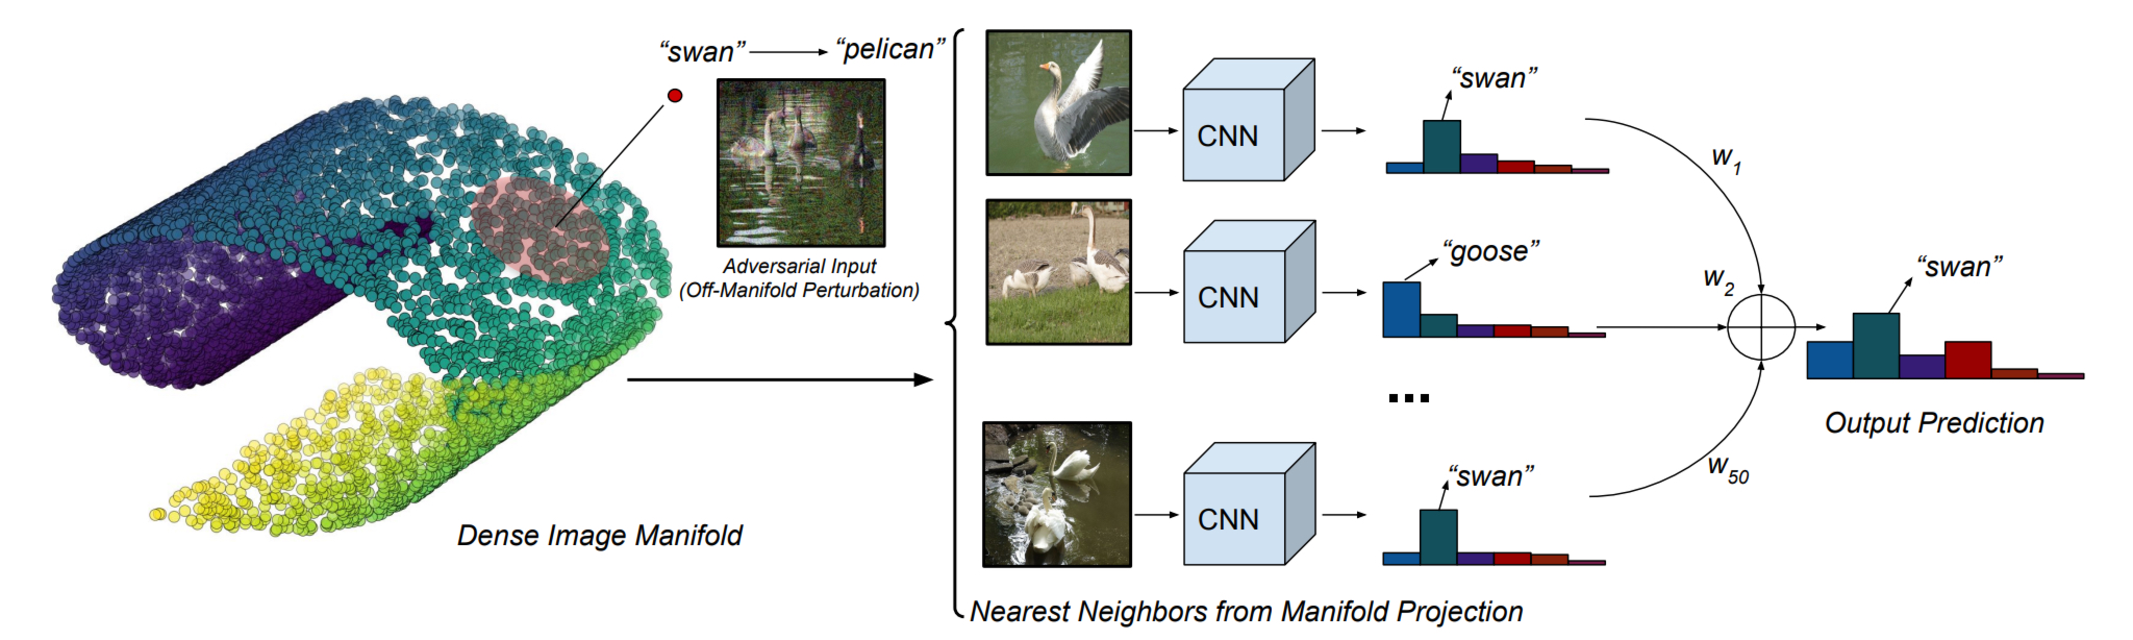
\includegraphics[width=16.0cm]{figures/defense-against-adversarial-summary.pdf}
\end{center}
\caption{
提案手法の概要図.
adversarial examples はそのままでは別クラスに予測されてしまうが, 外部データベースから似た画像を複数取得してそれぞれに対する確率値を重み付きで足し上げて最終的な予測とする.
図は \cite{dubey2019defense} より引用.
}
\label{fig:defense-against-adversarial-summary}
\end{figure}
%

この手法はモデルの softmax 値は adversarial examples で大きく影響は受けるが, 影響が比較的小さい中間層の特量量を使って似た画像を外部データベースから検索して引っ張ってくるという力技が特徴である.
画像検索技術の向上や大量データを含む外部データベースを豊富に活用している.

アルゴリズム自体に難しい点はなく, 検索して取得した $K$ 枚の画像に対する softmax 値をどのような重み $w$ で足すかのみを解説する.
まずは単純な平均で, Uniform Weighting (UW) と記す.
%
\begin{eqnarray}
w = \frac{1}{K}.
\label{eq:defense-against-adversarial-uw}
\end{eqnarray}
%
次に Confidence Based Weighting Entropy (CBW-E) で, softmax 値が一様分布からずれるほど大きくなるように重みをつける.
%
\begin{eqnarray}
w = \left| \log C + \sum_c^C f_{\text{prob}, c} (x) \log \left( f_{\text{prob}, c} (x) \right) \right|.
\label{eq:defense-against-adversarial-cbwe}
\end{eqnarray}
%
最後に Confidence Based Weighting Difference (CBW-D) で, $f_{\text{prob}} (x)$ を降順に並べた $\tilde{f}_{\text{prob}} (x)$ を用いて最大値との違いで重みづけをする.
%
\begin{eqnarray}
w = \sum_{m = 2}^{21} ( \tilde{f}_{\text{prob}, 1} (x) - \tilde{f}_{\text{prob}, m} (x) )^3.
\label{eq:defense-against-adversarial-cbwd}
\end{eqnarray}
%
ここで, $21$ や $3$ というような数字は予備実験で定めたパラメタである.

実験は ILSVRC2012 データを用いて, adversarial examples はステップ数が 10 の I+FGSM で作成する.
予測モデルとして ResNet-50 を用いる.
実験の設定として gray box と black box の 2 つを想定しており, 前者は adversarial examples を作成する際に前者は ResNet-50 をそのまま用いるが, 後者は ResNet-18 を用いる.
white box でなく gray box と呼んでいるのは, 画像検索の部分には感知せずに adversarial examples を作成しているためである.
論文ではこの画像検索部分の情報も使った攻撃手法も考案しているが, 本書では攻撃手法には立ち入らない.

典型的な結果は図 \ref{fig:defense-against-adversarial-result-table} である.
データ量が多いほど良い性能を発揮するようになるが, 闇雲に集めるのではなく予測対象となるラベルに近いものを選択的に集める方が良い.
重みに関しては CBW-D が良い結果を示しており, 絶対値で数 \% もの差が生じている.
kNN の検索には FAISS \cite{johnson2019billion} を用いている.
提案手法が有効であることは示されているが, clean データに対する性能は通常のモデルでは 80\% 程度が期待できるため, degradation は大きい.
%
\begin{figure}[htbp]
\begin{center}
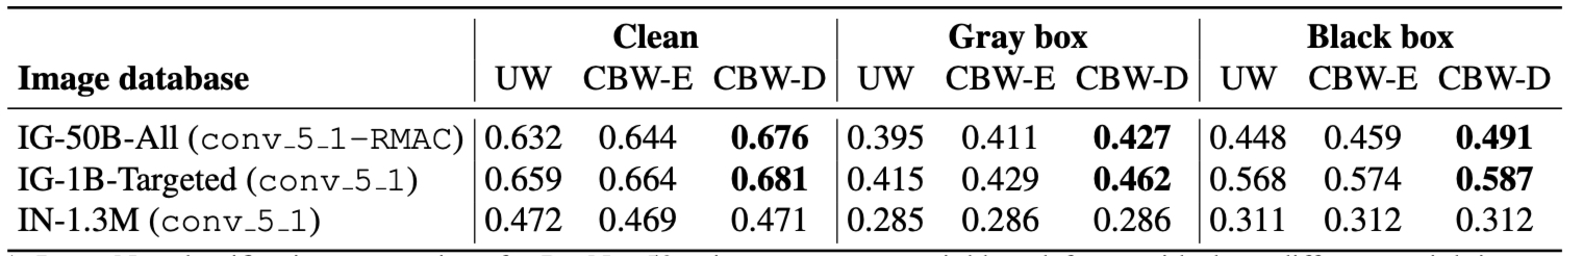
\includegraphics[width=14.0cm]{figures/defense-against-adversarial-result-table.pdf}
\end{center}
\caption{
ILSVRC2012 の validation データに対して I+FGSM で adversarial examples を作成し, 提案手法の正答率を測定した結果.
データベースは, 上から SNS で 500 億枚の画像をランダムに集めたもの, 真ん中が ILSVRC2012 の 1,000 クラスのどれか一つにはマッチする 1,500 個のハッシュタグに基づいて 10 億枚集めたもの, 下が ILSVRC2012 の約 130 万枚の学習データである.
データベースの横の括弧は検索時に使用する特徴量を記しており, RMAC は R-MAC pooling \cite{tolias2015particular} を意味している.
図は \cite{dubey2019defense} より引用.
}
\label{fig:defense-against-adversarial-result-table}
\end{figure}
%

この手法は新規性のあるアイデアというより, 外部データベースの大量の画像と画像検索という力技で防御を実現したものである.
所属期間の色もだいぶ出ている感じがするが, 実験も adversarial examples 系の論文としてはかなり大規模なものになっている.
摂動を無効化するために外部データベースに存在する他の画像を使うという点は興味深く, clean データに対する degradation も抑えられるような方向の発展が望まれる.
